\section{System Design and Implementation}
\label{sec:system-design}

% NB be more abstract in this section
% it sounds like you are talking about something that has already been made

% have a diagram of the system at the to
% following paragraphs explain the components
% any diagrams relating to those components go in these paragraphs as well

% explain why we use stuff in the introduction, give context

% explain how everything works in the respective subsection

% what does VRDAVis do
% it visualises large astronomy datasets
% using a server to store and process the data and a client to display the data and allow th user to interact and explore the data through a visualisation
% the server is accessible through the internet
% the client is also accessible through the internet
% the client functions within a web browser
% the client can function on a desktop computer such as a laptop or on a standalone VR headset such as the oculus quest 2

This section explains the design and implementation of the VRDAVis system. 
It outlines the system's structure and delves into how each component functions, some key language and package choices, as well as some key algorithms. 
The full source code can be found at the public GitHub repository for VRDAVis~\cite{VRDAVisGitHub}.

% libraries used in project
The architecture of CARTA was used as a guide for architectural choices and implementation. 
VRDAVis is a prototype proof-of-concept system, with the goal of potential integration into CARTA as additional functionality. 
The architecture was kept as similar as possible to allow the systems to be integrated with minimal changes to both systems.
% explain client-server architecture
%   server -> hosts, delivers, and manages most of the resources and services requested about the client
%   client -> presentation

% colour code diagram
\begin{figure*}
    \centering
    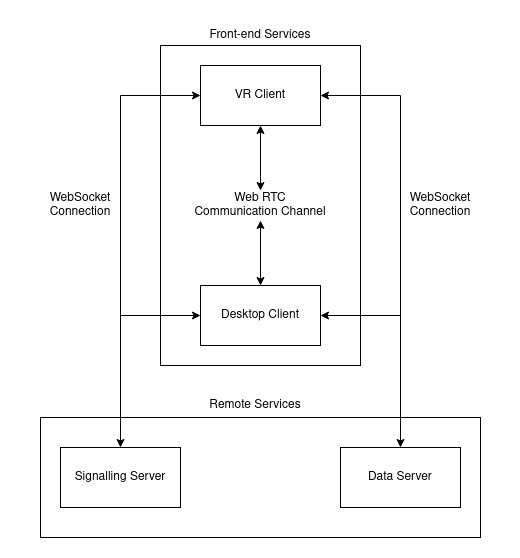
\includegraphics[width=0.6\linewidth]{figures/system-diagram.jpg}
    \caption{The VRDAVis high-level system architecture, showing the front-end and remote services. The arrows depict communication channels between the components, where the main channels of communication are between the client of the front-end services and the data server of the back-end services, the front-end client and the signalling server, and the VR and Desktop clients.}
    \label{fig:system-diagram}
\end{figure*}

The system uses the client-server architecture. 
With two main subsystems, the front-end and remote services.
The front-end service only contains the client web browser application.
This application is used on both the desktop computer and the standalone VR headset. 
These remote services host, deliver, and manage the resources and services requested by the client. 
% The data server and the signalling server sub-systems are separate remote systems which serve the client application. 
% The front-end services controls the majority of the system logic, while also being the main point of interaction between the data visualisation and the user. 

% The rendering approach, where a system like VRDAVis renders the data visualization on the client instead of the server, is referred to as client-side rendering. 
% A more in-depth explanation about the rendering approach can be found in Section \ref{rendering-strategy}.

Several libraries were evaluated for the development of VRDAVis. These included libraries for embedding VR environments and rendering three-dimensional graphics in a web browser, web-socket and peer-to-peer connections.
Aspects of these packages and libraries such as functionality, documentation, community support; must be considered before attempting to integrate.
Selecting a sub-optimal package which is not suited for the needs of the system could have potential cascading effects on the overall design of the system and the project timeline.
Many of the architectural and system choices were selected because for compatibility with CARTA's architecture, the relevance of each choice will be explain further in the respective sections.

% More details about the respective subsystems are explained in the sections below.

The main decisions in designing and implementing this architecture is deciding which system function are performed by the respective services. 
Once the system has been implemented, moving a task to a different service could be costly. 
For this prototype system, only one architecture could be tested, because of time constraints imposed on this research project.

% breifly explain the components of the system and how they work with each other
% the user side manages system logic and user interaction

The remote and front-end services, with their respective components, work together to create VRDAVis. 
We explain the functionality starting with front-end service, where the user begins their interaction with VRDAVis.

The web browser application is accessible through the Internet, either on a desktop computer or on a standalone VR headset. 
The interface allows the user to choose from a list of files available on the data server. 
These files are pre-processed HDF5 files that store data at various levels of resolution. 
This allows the browser application to request the same section of a data cube at a higher or lower resolution, and then display the requested data for the user to interact with.

The user can use the file selection UI on a desktop computer or a VR headset, but the embedded VR environment can only be accessed through the browser on the VR headset. 
Once the file has been selected, a low-resolution version of the entire data cube is requested from the data server. 
The data is sent from the data server to the browser application, where it is rendered into a visualisation. 
The visualisation can be viewed from the browser window or from within the VR environment.

However, if the user is viewing the visualisation from a desktop computer and would like to view it from a VR headset, the state of the visualisation can be transferred to the VR headset, and vice versa.
This process uses a peer-to-peer connection between the two devices to transfer the application's state. 
This connection is facilitated by the signalling server, which assists with the pairing of the devices as well as automatically establishing a new peer-to-peer connection. 
The signalling server itself is not involved with the data transfer once the connection is established.

Once the user has entered the VR environment, they can interact with the visualisation using various actions like translation, rotation, and scaling. 
If the user wants to examine a portion of the data cube in more detail, they can select the crop mode from the menu and draw a cube around the portion they are interested in. 
Once the area has been finalised and the crop button has been selected, the application determines which cubelets to request from the data server. 
As they arrive, they are reassembled into a larger cube and rendered. 
The user can continue to select and crop smaller portions of the visualised cubes until they reach the highest resolution level available for the selected file.

\subsection{Communication Layer}
\label{sec:communication-layer}
% introduction to communication layer
The sub-systems of VRDAVis need communication channels and protocols to communicate effectively.
These channels are established between the components of the front-end service and remote services. 
The data and signalling servers within the remote services communicate with the client application in the front-end. 
Peer-to-peer connections are formed between instances of the client within front-end services. 

\subsubsection{Data Server and Desktop/VR Client Application}
The communication between the user-side browser application and the server-side data server takes place through a WebSocket connection, which is more suitable for VRDAVis than the typical request and response or promise and resolve model common in many HTTP-based clients and servers~\cite{MDN_WebSockets_API}.
WebSockets allow the respective systems to send messages to each other without requiring a request first to respond. 
This behaviour allows for many responses to a single request, 
so the server is not restricted to responding to the client with a single very large message with a large piece of data, it can send smaller pieces of data in individual messages.

Protocol Buffers are used to define the structure of messages and facilitates the reading and writing of structured data to and from various data streams using different programming languages, such as C++, JavaScript, and Python.
The Protocol Buffer library was created by Google to serialise structured data. 
A platform-neutral mechanism for converting data objects into a byte stream for transfer~\cite{Google_Protocol_Buffers}.
This library is used to define a schema and format for data exchanged between the front-end and remote services. 
The Protocol Buffer message definitions are stored in their own folder and are used by the user-side and server-side systems. 
When a message needs to be sent from the user-side to the server-side or vice versa, the data objects are serialised into a byte stream before they are transferred. 
Once the data arrives, it is converted from a byte stream back into a data object.
% serialisation -> process of converting data type objects into a byte stream for transfer
IProtocol Buffers was chosen for its error-prevention capabilities compared to JavaScript Object Notation (JSON), and because it is the chosen communication format used in CARTA.

\subsubsection{Signalling Server and Desktop/VR Client Application}
The signalling server creates, manages, and establishes peer-to-peer connections between instances of the client browser application on different devices.
% JSON
The communication required between the signalling server and the client application is significantly less complex than the communication between the data server and the client application.
The tasks performed by the signalling server are also less time-sensitive than those performed by the data server, and less data needs to be transferred between them.
These factors led to the use of the simple request-response communication protocol to be used as well as the use of JSON to format the messages.
JSON is a lightweight format for storing and transporting data that is language-independent and easy to understand as it considered ``self-describing"~\cite{JSON}.

\subsubsection{Client Application and Client Application}
Another component of the communication layer is the peer-to-peer connection between two instances of the client web browser application. 
One of these instances would be in a browser on a desktop computer, and the other would be in the browser on a standalone VR headset. 

Web Real-Time Communication (WebRTC)~\cite{Blum2021, WebRTC} is an internet communication protocol that enables web applications to stream audio, video, or data between peer browser windows, without the need for the data to be routed through an intermediate server. 
It facilitates peer-to-peer communication without requiring additional third-party packages.
% facilitates peer-to-peer without requiring plug-ins or third-party software to be installed
% support for audio and video conferencing, file exchange, screen sharing, identity management, and interfacing with legacy telephone
WebRTC is used in VRDAVis to establish a connection between these instances. 
This connection is used to transmit the application's state between its peers, allowing the user to continue their work seamlessly without needing to repeat steps on another device.
% used to create a peer-to-peer connection between browser instances on different devices
% used to send data between the broswer instances 
% chosen for its functinality to create peer-to-peer connections
% peer-to-peer connection
This peer-to-peer connection allows the instances to exchange data between instances without having to send it through middleware service such as a server. 
However, it does require the signalling server to establish and manage the connections. 

% has the capability with help from the signalling server to create a peer-to-peer conection between another instance of the client on a VR headset
%   show pairing process diagrams
%   show transfer diagram

\paragraph{Headset Pairing}
% To establish the connection both devices must connect to the signalling server which a server-side component which stores unique id pairs which.
The initial pairing process requires both of the VR headset and the desktop computer to be connected to the signalling server. 
When each devices connects, it sends the server an unique ID, a name, and announces whether it is a VR capable device. 
The server checks if the device already has a pair and if it does not find a pair it sends a list of unpaired VR devices to the unpaired devices which are not VR-capable. 
A desktop user selects a VR device and generates a code from the desktop computer, a code which is sent to the signalling server, and forwarded to selected device using its unique ID. 
The VR device then prompts the user to enter the code locally, and verifies it against the code received from the server.
When the server confirms that the codes match it saves the device pair to a local JSON database.
The server then sends a confirmation message to both devices stating that the devices have been paired.
Both devices then confirm that they are ready to begin a peer-to-peer connection and the WebRTC peer-to-peer protocol begins.

\begin{figure}
    \centering
    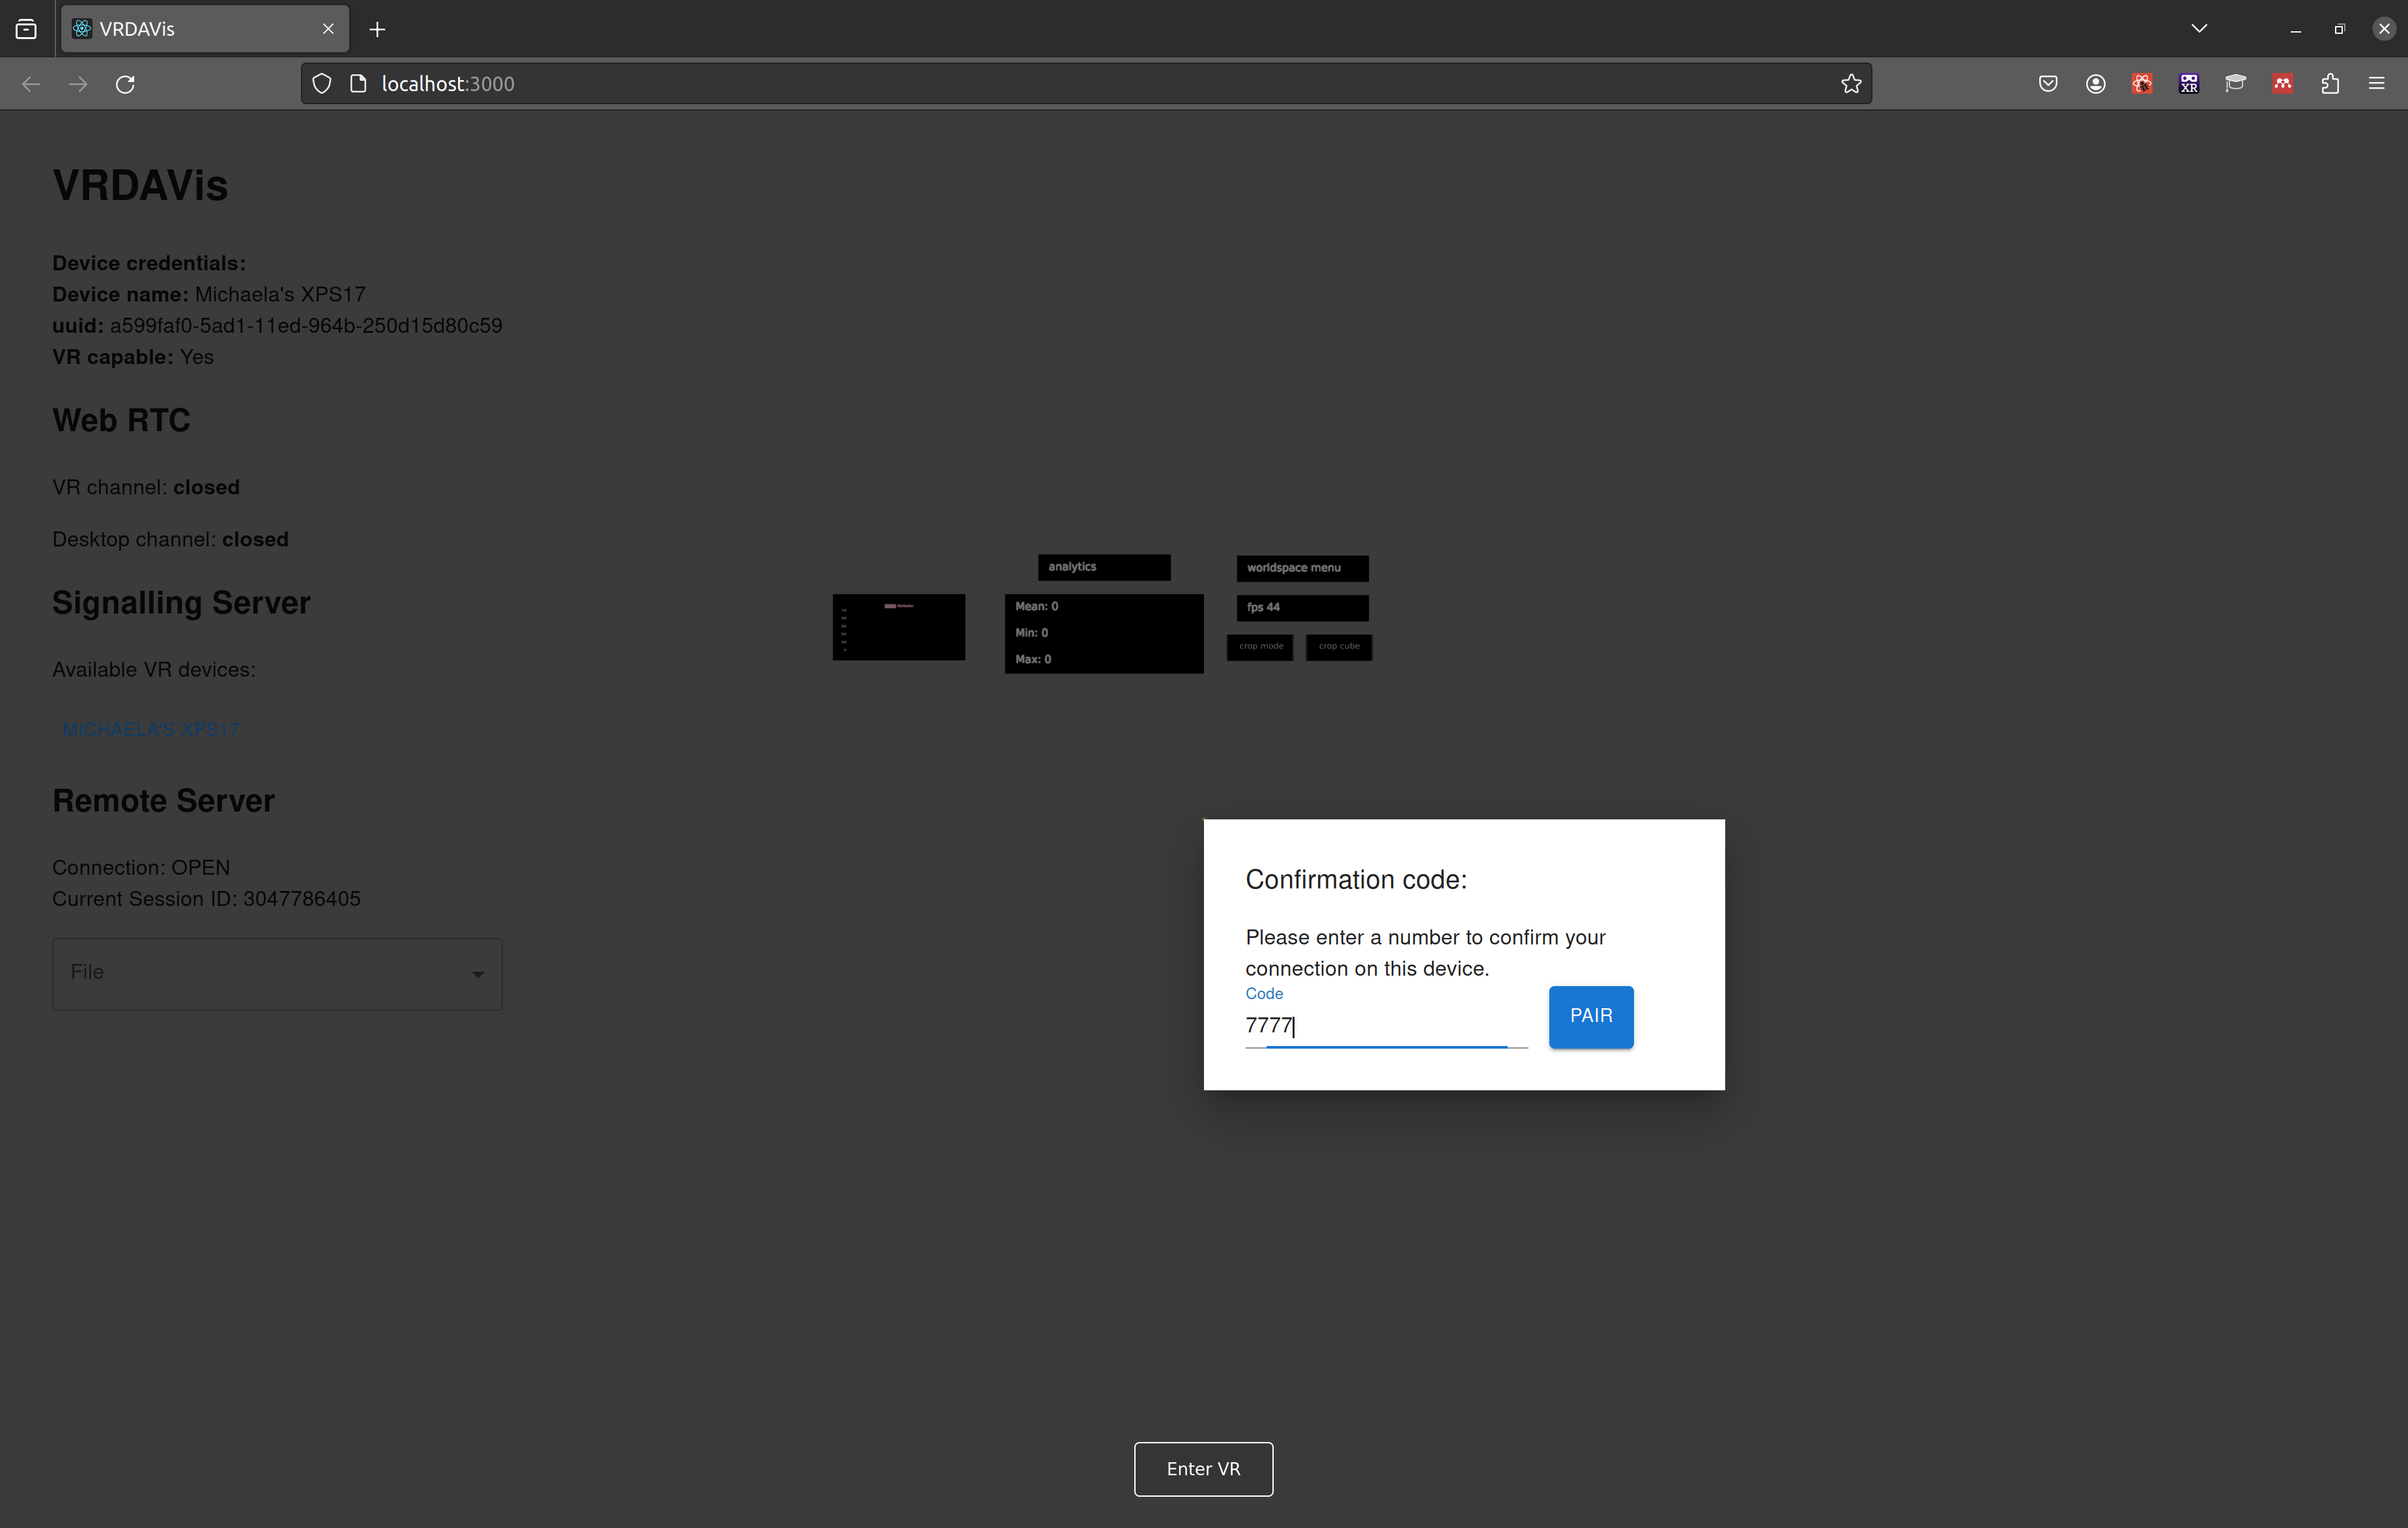
\includegraphics[width=\linewidth]{figures/screenshots/3.png}
    \caption{The menu that appears in the browser window when the user selects a VR device to pair with on the desktop computer. The user must enter a code which must also be entered in the same menu on the VR headset.}
    \label{fig:screenshot-3}
\end{figure}

% pairing process diagrams
\begin{figure*}
    \centering
    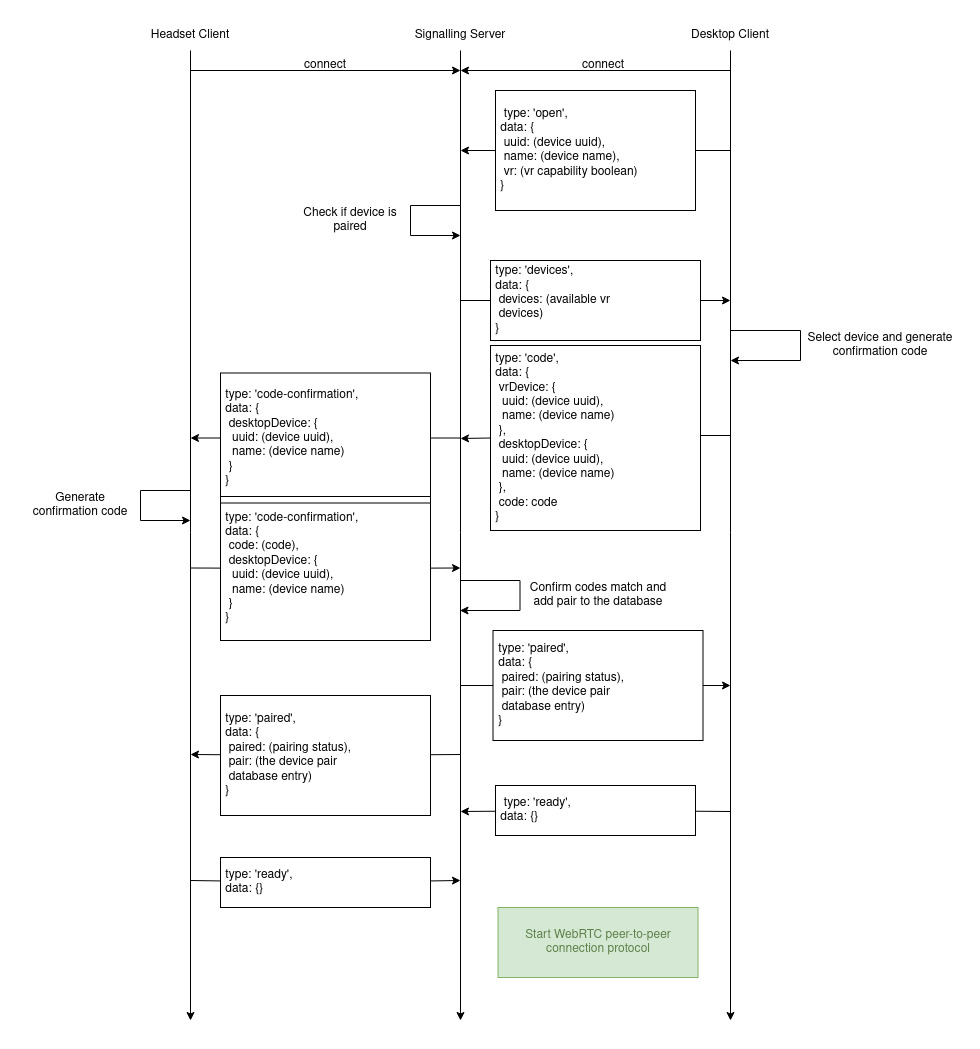
\includegraphics[width=0.6\linewidth]{figures/pairing-process.jpg}
    \caption{The pairing process between an instance of the front-end application running on a desktop computer and an instance running on a VR headset. It shows the order of the messages sent from each device and the contents of each message.}
    \label{fig:pairing-process}
\end{figure*}

\paragraph{Paired Devices Connection}
% Once the devices have been paired they must connect to the signalling server at the same time and then a peer-to-peer connection is established between the paired devices. 
% No data which is sent between the devices on the peer-to-peer connection passes through this server.
When one device connects to the signalling server, the server checks if the device is currently paired by searching the JSON file which contains all the pairs.
If the device is paired, the server checks if the other paired device is connected to the server as well.
When the VR device and the desktop computer are connected to the signalling server and the server detects that these device are paired to each other, it starts the process of creating the WebRTC peer-to-peer connection.

\begin{figure*}
    \centering
    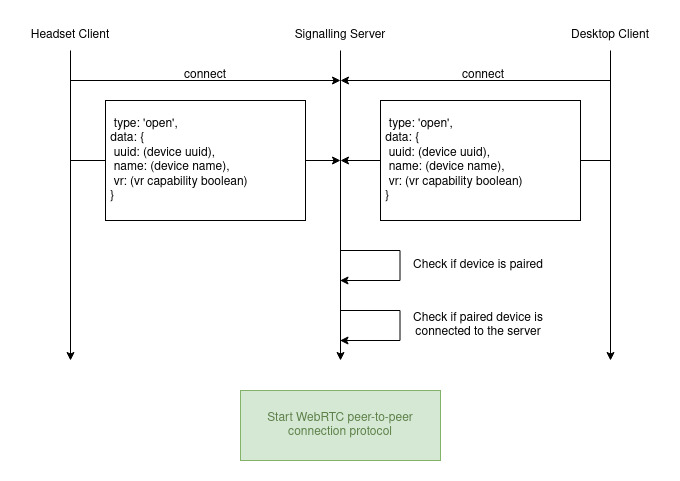
\includegraphics[width=0.6\linewidth]{figures/connect-paired-devices.jpg}
    \caption{The process of connecting paired devices through the signalling server. Both devices indicate that they wish to open a peer-to-peer connection with their ``open" messages.}
    \label{fig:connect-paired-devices}
\end{figure*}

\paragraph{Peer-to-peer Connection}

Once the VR headset and the desktop client indicate that they are ready to establish a peer-to-peer connection with each other,
the desktop client sends WebRTC Interactive Connectivity Establishment (ICE) candidates to the VR device through the signalling server.
These ICE candidates contain the protocols and routing needed for remote devices to communicate with each other as well as details used to establish the connection.
Multiple candidates are sent until one is found which works for both devices.
The candidates are sent to the VR device through the signalling server as this is the only channel currently connecting the devices.
The desktop computer creates a Session Description Protocol (SDP) offer, which contains the RTCPeerConnection interface. 
It contains information about open channels already attached to the current WebRTC session, a codec, any candidates already gathered, and options supported by the browser.
This SDP offer is sent to the VR device through the signalling server, and the VR device handles the offer through WebRTC by creating an answer which contains the corresponding information about its own capabilities.
The answer is returned to the desktop client, the offer is resolved and the peer-to-peer connection is established between the devices.
No further data needs to pass through the signalling server in order for the devices to communicate with each other; they now pass data to one another through the peer-to-peer connection.

\begin{figure*}
    \centering
    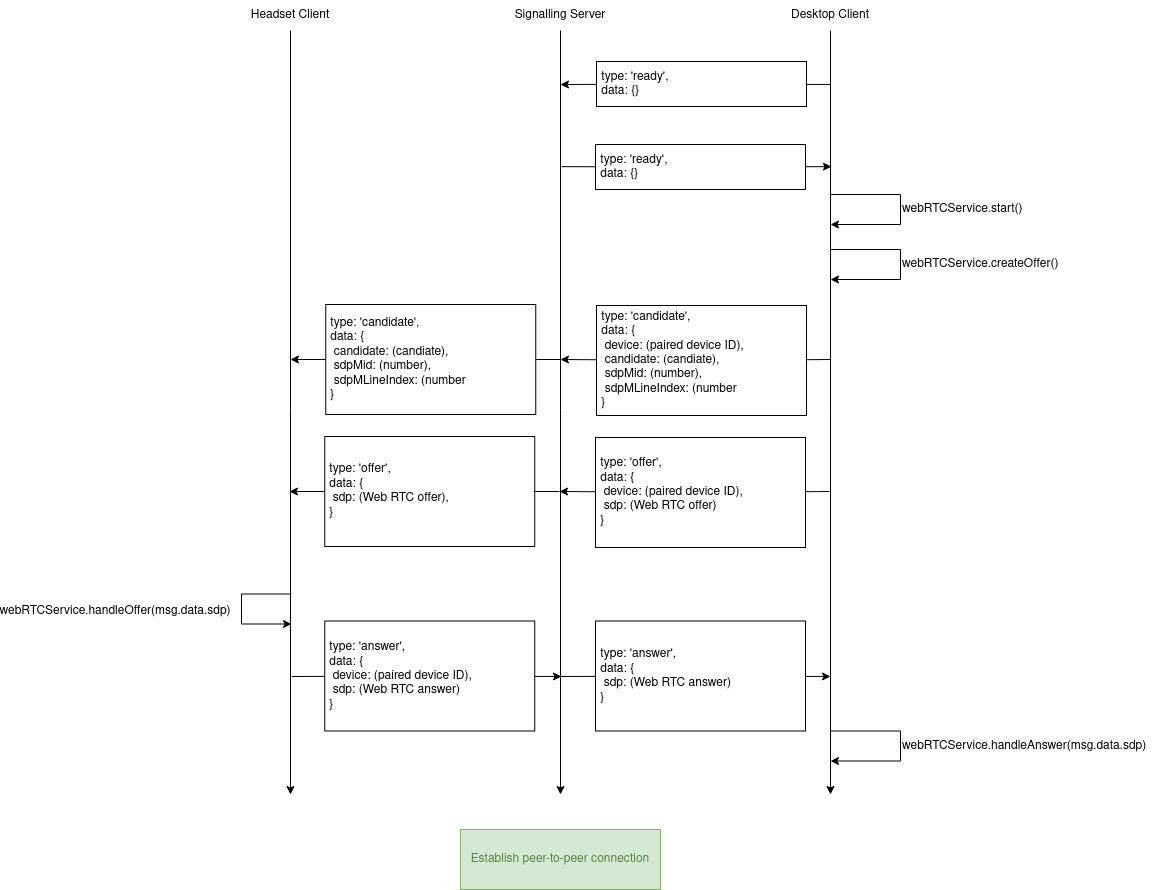
\includegraphics[width=0.8\linewidth]{figures/peer-connection(1).jpg}
    \caption{How the peer-to-peer connection is established between the paired devices.}
    \label{fig:peer-connection}
\end{figure*}

\paragraph{Transferring Client Application State Over Peer Connection}
The purpose of the peer-to-peer connection is for the connected instances of the front-end to exchange state.
This allows the user to start their exploration of a data cube on a device such as a laptop or a desktop computer, then move the state of the desktop instance to the VR headset to continue the exploration in the VR environment.
Transferring the state of an instance in this manner means that the user does not need to perform additional steps to start a new instance and get back to the same position in their new exploration.

The state is transferred through JSON messages sent over the peer-to-peer connection.
Each message contains the file name, and the size and the position of the local cube state.
Once these details have reached the new instance, a new connection to the data server is used to make requests and receive responses from.

% JSON
% add a diagram for how the state is transferred between the devices
\begin{figure*}
    \centering
    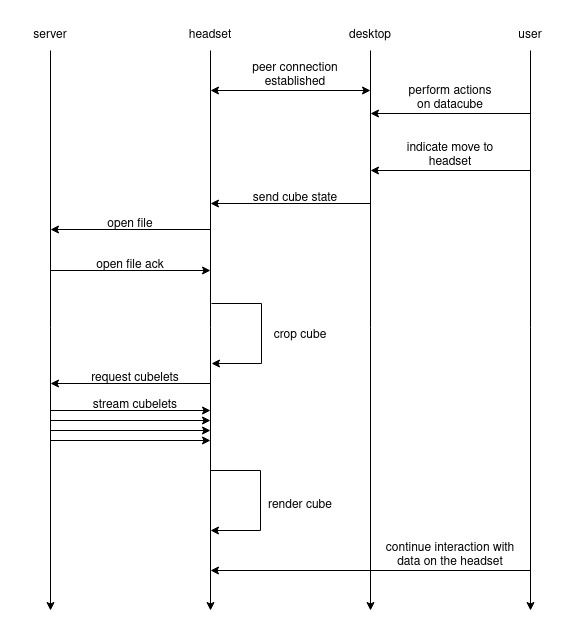
\includegraphics[width=0.6\linewidth]{figures/transfer-flow.jpg}
    \caption{The diagram depicts the event sequence for transferring the state between the two instances of the front-end browser application. The application state can be bilaterally transferred between client devices.}
    \label{fig:transfer-flow}
\end{figure*}

\begin{figure*}
    \centering
    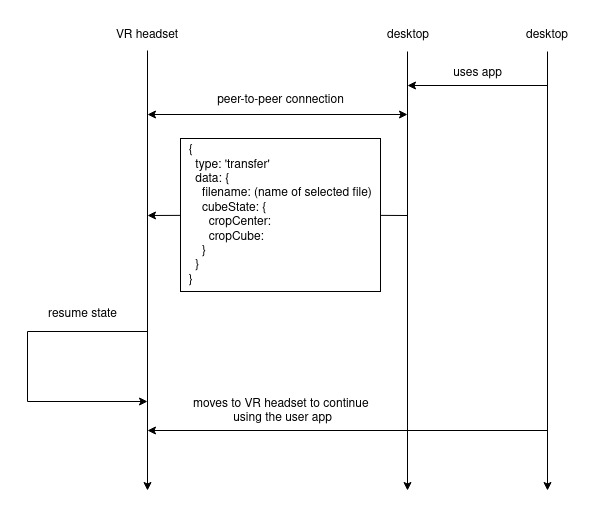
\includegraphics[width=0.6\linewidth]{figures/transfer-cube-state.jpg}
    \caption{The message structure which is sent between the VR headset instance and the desktop instance when the cube state needs to be transferred between the devices.}
    \label{fig:transfer-cube-state}
\end{figure*}

\subsection{Server-side}
\label{sec:remote services}

The remote services of VRDAVis are composed of all the systems that serve the front-end applications; consisting of a data server and a signalling server. 
The data server receives requests from the user application, where its purpose is to transfer data from astronomy data files. 
The signalling server is used to create and manage peer-to-peer connections between two instances of the front-end browser application. 
The peer-to-peer connection is used to transfer the state of the visualisation across instances, allowing the user to transfer the state from a desktop computer to a standalone VR device and vice versa. 
This showcases how VRDAVis would be able to integrate into an astronomer's workflow with minimal disturbance.
% The main purpose of the server-side systems is to serve requests from the front-end clients. 

\subsubsection{Data Server}
% preprocessed files
% cite the CARTA HDF5 papers
% point out that there is a converter from FITS to HDF5
It is common in astronomy for data to be stored in the FITS format.
But in VRDAVis the HDF5 file format will be used to store data. 
Unlike FITS files, where data must be read sequentially, the HDF5 format allows any part of the file to be accessed at any point in time. %cite
The HDF5 C++ library is used to read the files. 
Initially written in C, the C++ package encapsulates the Python code into a format that can be interfaced with C++.

However, merely using a more effective file type is not provide speed-up for creating a visualisation of the stored data. 
Especially when the data in the file is still at its original resolution and therefore its largest size. 
It has the potential to overwhelm the client device with the sheer amount of data it would need to process.
The full-resolution data must be processed into multiple levels of resolution, referred to as mipmaps. 
These mipmaps are contained in the same HDF5 file as the data at its original resolution. 
Portions of the mipmaped data are read, instead reading the full-resolution data, decreasing the likelihood of overwhelming a client device.
% mention that the FITS to HDF5 converter also does the mipmap conversions
% cite the git repo

The server stores the data files pre-processed into a mipmaped format.
This approach to handling \textit{Big Data} files allows the entire dataset to be visualised with less computational overhead, compared to rendering the full resolution dataset~\cite{Li2016}. 
It still allows the visualisation to maintain the overall context of the data, but as the data is explored, higher resolution versions of the same region can be swapped out to allow the user to observe the details.

% insert diagram of how the preprocessed cubelets are stored in the server
\begin{figure*}
    \centering
    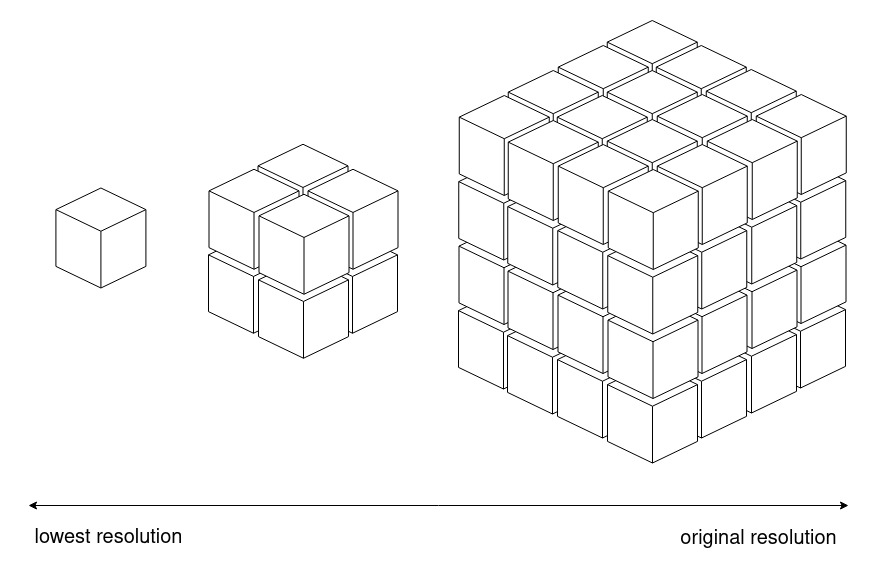
\includegraphics[width=0.6\linewidth]{figures/three-dimensional-mipmap.jpg}
    \caption{In the pre-processed data file, different resolutions are stored as mipmaps, from a single cubelet which represents the entire data cube to the original full-resolution data, with several intermediate levels.}
    \label{fig:three-dimensional-mipmap}
\end{figure*}

\begin{figure*}
    \centering
    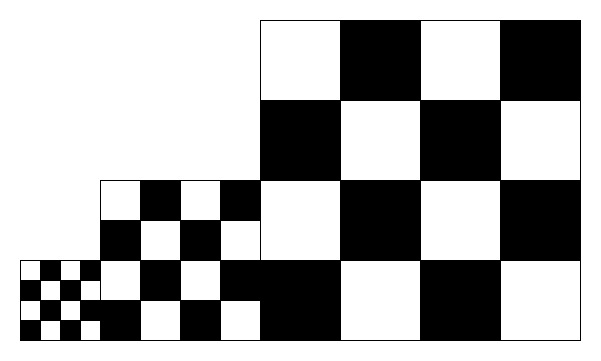
\includegraphics[width=0.5\linewidth]{figures/two-dimensional-mipmap.jpg}
    \caption{An example of a two-dimensional mipmap. Observe how the pattern is scaled at each level}
    \label{fig:two-dimensional-mipmap}
\end{figure*}

% mipmap
% \cite{Li2016}
% The displays on which the visualisations are rendered have a limited number of pixels, thus the lowest granularity possible is to plot one data point onto one pixel (Molina-Solana et al.2017; Olshannikova et al.2015; Yang et al.2015). 
% Visualisation tools are required to “squeeze a billion records into a million pixels”(Bikakis2018) empha-sizing the need for summarisation of data, particularly when creating visualisations

The server must fetch data from its filesystem according to the client's request. 
When the client requests a number of sub-sections of a data cube, the server retrieves these cubes or cubelets and streams them back to the client over a websocket connection. 
Each message streamed to the client contains one compressed cubelet. 
Additionally, the server performs file system functions such as sending lists of available files, opening them, and reading data.

The ability to view various analytics on the visualised data is also an important feature, and the server supports this by computing various derived values such as minimum, maximum, and median values. 
It also compiles analytics data to be visualised as various graphs, including the distribution of values.
%   fetches data based on the client's request
%       client requests a number of cubes but the server streams back the data in chuncks 
%       each message back to the client has the data of a single cube contained within it
%   file system functions (opening files and reading data from them)
%   performing analytics functions on data
% stores the data
%   the pre-processed mipmap data cubes as well as the full sized data cubes

The data server was written in C++ for the purposes of speed and performance and follows a similar structure to the CARTA software.
C++ is a high-level, general-purpose programming language used to implement the data server of VRDAVis remote services. 
An object-oriented programming language that was initially released in 1985 as an extension of the C programming language, with a focus on performance, efficiency, and flexibility.

It was selected for its speed of execution and object-oriented nature, as well as being the same language utilised in implementing the CARTA back-end.
uWebSockets is a C++ library used to integrate WebSockets into a C++ project.
It is also used establish WebSocket connections between the client application and the data server.

\subsubsection{Signalling Server}
Node.js, also referred to as Node, is a free, open-source server environment, with cross-platform capabilities, which uses JavaScript to create server-side tools.
It uses asynchronous programming which is a different manner to handle the conventional HTTP one request, one response model.
Synchronous systems wait for tasks to complete before returning content to the client, only once a task is complete is the system ready to handle the next request.
Asynchronous systems do not wait for a task to be completed before starting a new request.

VRDAVis uses Node in the signalling server to create and manage peer-to-peer connections between the instances of the front-end web applications.
It was chosen because servers can be implemented quickly.

Express is a minimal and flexible Node.js framework that provides a robust set of features for the development of web and mobile applications.
It is one of the most popular Node web frameworks.
% cite
It provides functionality to write handlers for HTTP requests at different URL paths know as routes.
It is integrated with view-rendering engines, which generate responses by inserting data into templates.
It has the functionality to set common web application settings like the connection port, and the location of templates.
It can also insert additional request processing known as middleware at any point within the request handling pipeline, to add functionality such as authentication.
It is used in the VRDAVis signalling server to implement the WebSocket connections, and was chosen because of its flexibility and the speed at which prototype systems can be implemented.

% from the comm section
% This server-side component is named the signalling server and is made using Node.js and JavaScript. 
% It also uses a WebSocket connection to communicate with the web browser application and sends dats using JSON. 
% Unlike the data server, this server component was not made with speed and performance as its main focus. 
% The speed of implementation was the focus when creating this component. 
% Its main purpose in the context of the VRDAVis system, besides creating the peer-to-peer connections, is to pair the devices, store the devices pairs, and streamline the connection process when the pair needs to reconnect.
\subsection{User-side}
\label{sec:user-side}
% give an overview of the user-side system
% a web browser application
The front-end service of the system is a user serving web browser application accessible through the internet. 
The decision to use a browser application ensures that application is operating system-agnostic, which makes it available to more user devices. 
It also allows the system to remain up-to-date with any changes for all users, unlike native applications, which the user is responsible for updating. 
% The front-end application is used on desktop computers and standalone VR headsets. 
The instances of the application can be used on desktop computers, laptops, and standalone VR headsets, and communicate through a peer-to-peer connection, which allows them to coordinate with each other without routing data through a server. 
These web application instances serve as entry points to the embedded VR environment, which can be accessed through the VR headset. 
This is the environment where the user can see the visualised data, interact with the visualisation, manipulate it, and explore.

React.js is the framework chosen to implement the web application for VRDAVis, to replicate architectural choices from the CARTA system, as CARTA also uses React.js for its front-end application.
It is a free and open-source JavaScript library is used for building user-oriented applications based on components and can be employed to develop single-page, mobile, or server-rendered applications. 
It is maintained by Meta and a community of individual developers as well as companies.

In addition to React.js, MobX is a state management library designed for front-end web browser applications, responsible for maintaining stateful information. 
It integrates into React and is also used for state management within the CARTA framework.

% explain how the mipmap data supports functionality on the front-end
% no unneccessary rendering of points which equate to smaller than a pixel
% it returns a managable amount of data
% does not overwhelm the computer with the sheer amount of data it needs to process

% hosts some of the system logic
The front-end also hosts the majority of the system logic as it determines which piece or pieces of data need to be retrieved from the server. 
When the initial data is retrieved or the cube is cropped, a list of cubelets must be made so that the correct subsections can be fetched from the appropriate resolution level. 
The resolution level and lists are determined through a selection process taking into account the predetermined cubelet size, cubelets are selected from a mipmap level which maximises the resolution while maintaining performance. 
It is biased towards the mipmap layer with the maximum downsample ratio, which reduces the total number of cubelets that cover a selected area, whether it is the whole cube or a subset of the cube. 
This strategy limits the maximum amount of data that can be sent to the client. 

This selection process is critical when the cube is cropped on the front-end, as it discards portions of the cube that are not being focused on. 
Figure \ref{fig:crop-cube} illustrates the relationship between the cropped portion of the cube and the cube space, showing the dimensions of the full-resolution cube, as well as how multiple cropping actions relate to each other. 
Each crop action selects a subset of the previous cube.

The algorithm used to crop the cube and select cubelets at a higher resolution level can be broken down into the several steps:
\begin{enumerate}
    \item To determine which cubelets need to be requested initially, the full-sized data cube is cropped with a selection boundary of the same size.  The cube localspace is the current state of the cube being visualised on the front-end application, and the crop cube is the subset of the cube for which higher resolution cubelets are going to be requested.
    \item Every time the cube is cropped, the visualised cube's space and crop cube's space are aligned in the full-resolution cube's space, which can also be referred to as the cube's worldspace, encapsulating the full resolution dimensions. This is done to ensure that the crop cube's corner coordinates fall within the x, y, and z dimensions of the cube's coordinates. This is achieved through the multiplication of the crop cube dimensions and the centre coordinates by the current mipmap level. The initial mipmap level for the XY and Z axes is set to 1, and when the cube is cropped, the cube localspace dimensions and centre are updated to equal the crop cube's dimension and centre.
    \item The corners are calculated by the division of the dimensions by 2 then the addition or subtraction of this number to the centre for the x, y, and z dimensions.
    \item The crop cube's dimensions and centre are translated to coordinates within the full-resolution cube.
    \item The maximum mipmap level that data can be fetched from is determined by the adjustment of the crop cube corners to coordinates within the data cube, so that the centre of the axis shifts from zero to the midpoint of the full-resolution cube dimensions. This point is referred to as the adjusted centre.
    \item The current mipmap for XY and Z is initially set to 1. The minimum and maximum values of x, y, and z dimensions are determined to establish which cubelets are fully or partially inside the cropped area.
    \item The crop cube dimensions are rounded to the nearest cubelet boundary. 
    \item The process then steps through each range from the minimum boundary to the maximum boundary level. 
    \item The step is divided by the cubelet dimension size to determine the encoded coordinate of the cubelet needed from the data server.
\end{enumerate}
% mipX = Math.pow(2, Math.ceil(Math.log2(this.cropCube.x * this.currentXYMip)))/CUBELET_SIZE_XY;
% mipZ = Math.pow(2, Math.ceil(Math.log2(this.cropCube.z)))/CUBELET_SIZE_Z;
% Where the begining and end of each dimension of the cube in mipmap level is determined by
% const xStart = Math.floor((cubeState.xMin / cubeState.mipXY) / CUBELET_SIZE_XY) * CUBELET_SIZE_XY;
% const xEnd = Math.ceil((cubeState.xMax / cubeState.mipXY) / CUBELET_SIZE_XY) * CUBELET_SIZE_XY;
% \[ maxmip_x = 2^\frac{\cdot{cropCube_x}{currentMip_x}}{cubelet_x} \]

\begin{figure*}
    \centering
    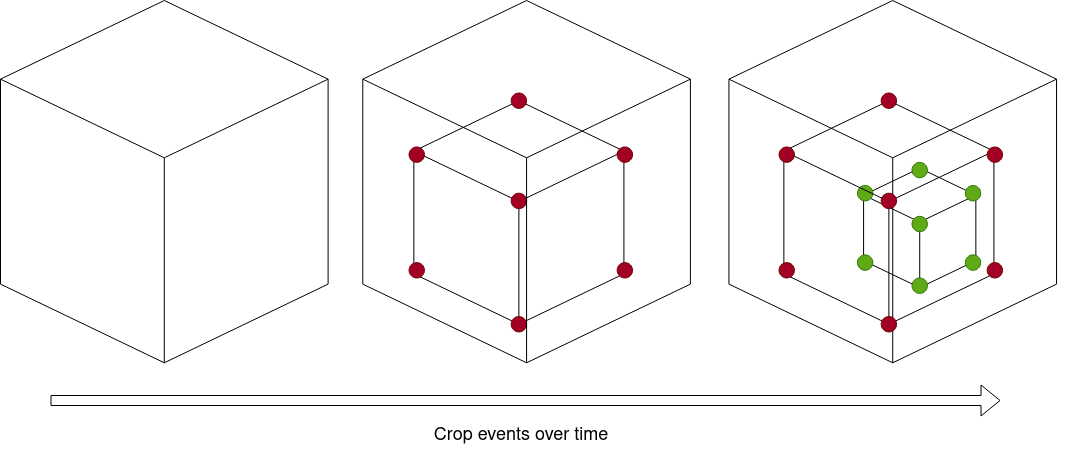
\includegraphics[width=0.6\linewidth]{figures/crop-cube.png}
    \caption{The relationship of the crop cube across cropping events to the full resolution data cube as the user drills down into a section of interest. The cropped sections refer to the marked red and green squares in the diagram; these sections are a selection made during a crop action. They are the portion of the data used to create the visualisation in the front-end services.}
    \label{fig:crop-cube}
\end{figure*}

% Virtual Reality Environment
% As the popularity of VR has boomed in recent times, there have been major developments in VR technology, driven by the demand for VR devices in the entertainment industry ~\cite{Farr2009}. 
% The virtual reality component of the front-end is embedded in the web browser application, and with packages like Three.js and WebXR, VR and three-dimensional environments can be embedded into web pages. 
WebXR grants access to the display of the headset, as well as the positions of the camera and controllers, allowing for integration with the web. 
Three.js was used to create the assets within the VR environment, such as the data cube used to display the astronomy data, and the UI elements which use canvases as textures to display text on a plane. 
These elements are made interactive through WebXR functions. 
The combination of these libraries facilitates a VR experience through the internet.
The data visualisation is presented within the VR space as a cube mesh with a three-dimensional texture used to map the three-dimensional data. 
This presentation method was selected because of its minimal processing cost~\cite{Ferrand2018}.
% choice to use volume rendering
%   present the data as is with minimal processing
%   iso-surface models must be generated using the raw data

% performs the rendering of the data
The data visualised by VRDAVis is volumetric astronomy data; however, this system would be able to visualise any volumetric data as long as it is in the HDF5 file format.
The HDF5 schema used is the same schema used by the fits2idia repository~\cite{fits2idia}, which is used to convert FITS files into the HDF5 files.
The mipmaps in the HDF5 file are stored according to their downsampling ratios.
For example XY\_2\_Z\_4 means that the x and y axis have been downsampled to a size 2 times smaller than the original cube and the z axis has been downsampled 4 times smaller than the original cube. 
The data arrives at the front-end from the data server in a float array format, where it is placed in a three-dimensional texture and rendered using a ray-cast shading technique.
The process of the ray-casting shader has the following steps:
\begin{enumerate}
  \item A ray is cast until it hits a bounding box of the volume texture.
  \item The ray takes a step through the volume and samples a point from the three-dimensional texture.
  \item The values that the ray sampled are added to an accumulator to determine the opacity of the pixel.
  \item The shader keeps track of the maximum value the ray has sampled.
  \item The ray continues to sample points until it has reached its maximum step count or the accumulated opacity reaches a 100\%.
  \item The shader then samples a two-dimensional colour map texture to retrieve a colour value for the pixel.
  \item If the opacity of the pixel is 0\%, the point is discarded.
\end{enumerate}

The rendering of the data with a ray-casting shader was implemented with the Three.js framework~\cite{Danchilla2012}, it can be easily integrated with React.js, a cross-browser JavaScript library built on top of WebGL. 
It is used to create and animate three-dimensional computer three-dimensional graphics within web browsers.
Three.js is widely adopted, and benefits from an active community that offers robust support. 

The shader goes through these steps for every frame, for every pixel on the screen. % cite
This is the most computationally expensive step in the visualisation process. 
Although ray-cast shading is computationally expensive, it depicts the data in a way that closely matches its structure, as if it were a high-resolution three-dimensional scatter plot.

For the user to view the visualisation with the VR headset in a virtual environment, a package is require which makes the three-dimensional environment compatible with VR displays and controllers.
WebXR provides access to input data related to the pose information from the headset and controllers, and output, which is the display within the headset. 
This technology enables web browsers to facilitate Virtual Reality (VR) and Augmented Reality (AR) experiences over the internet. 
It encompasses functionalities commonly associated with VR and AR devices.

In VRDAVis, WebXR is used to integrate an embedded VR environment into the client web application. It works in conjunction with Three.js and React.js to create an immersive three-dimensional environment, constituting the VRDAVis front-end application.

\subsubsection{User Workflow}

\begin{figure*}
    \centering
    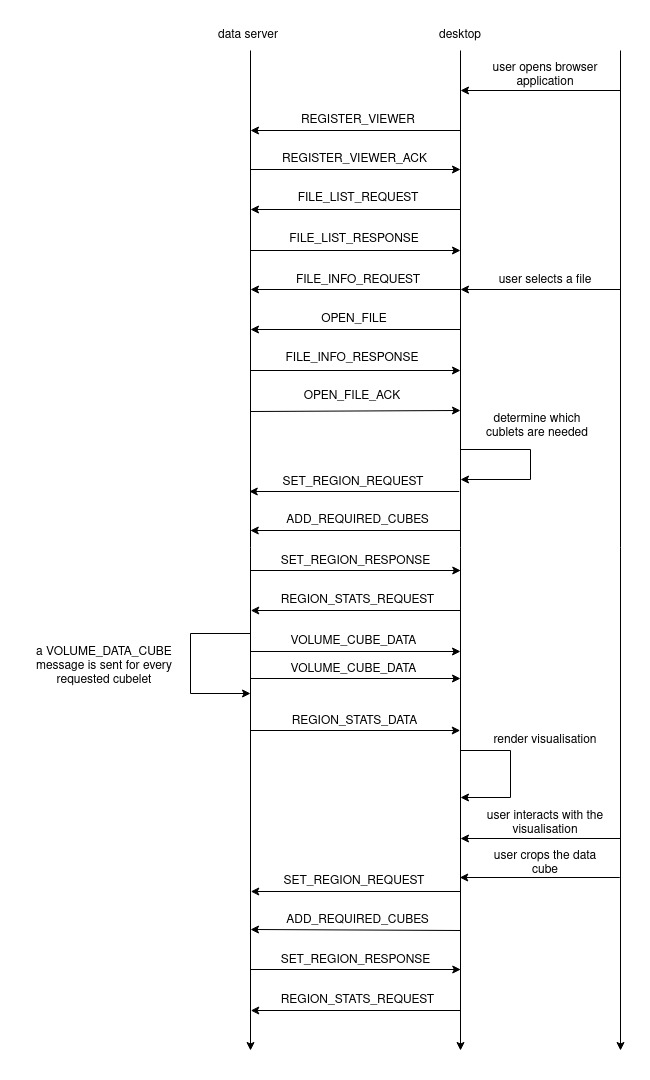
\includegraphics[width=0.6\linewidth]{figures/user-worklow(4).jpg}
    \caption{ A sequence diagram showing the user's interaction with an instance of the client application and the corresponding protocol buffer messages which are sent from the front-end to the back-end, as well as the responses from the back-end to the front-end. It shows the message sequence of the user opening the front-end application, selecting a file from a list, and cropping the visualisation.
    }
    \label{fig:user-workflow}
\end{figure*}

The user first opens an instance of the browser application on their desktop computer. 
When it is launched, this application instance creates a connection with the remote services such as the data and signalling servers. 
The signalling server connects the desktop client instance and pairs with the standalone VR headset if it is also connected to the signalling server at that time. 
This connection is made automatically once both devices are connected to the server. 
If the desktop device is not paired, then the user can pair it with an available unpaired device. 
When this peer-to-peer connection is created, the state of the visualisation can be transferred between the paired devices. 
The data server acknowledges the client application's connection, and the client requests a list of the available files on the server.

\begin{figure}
    \centering
    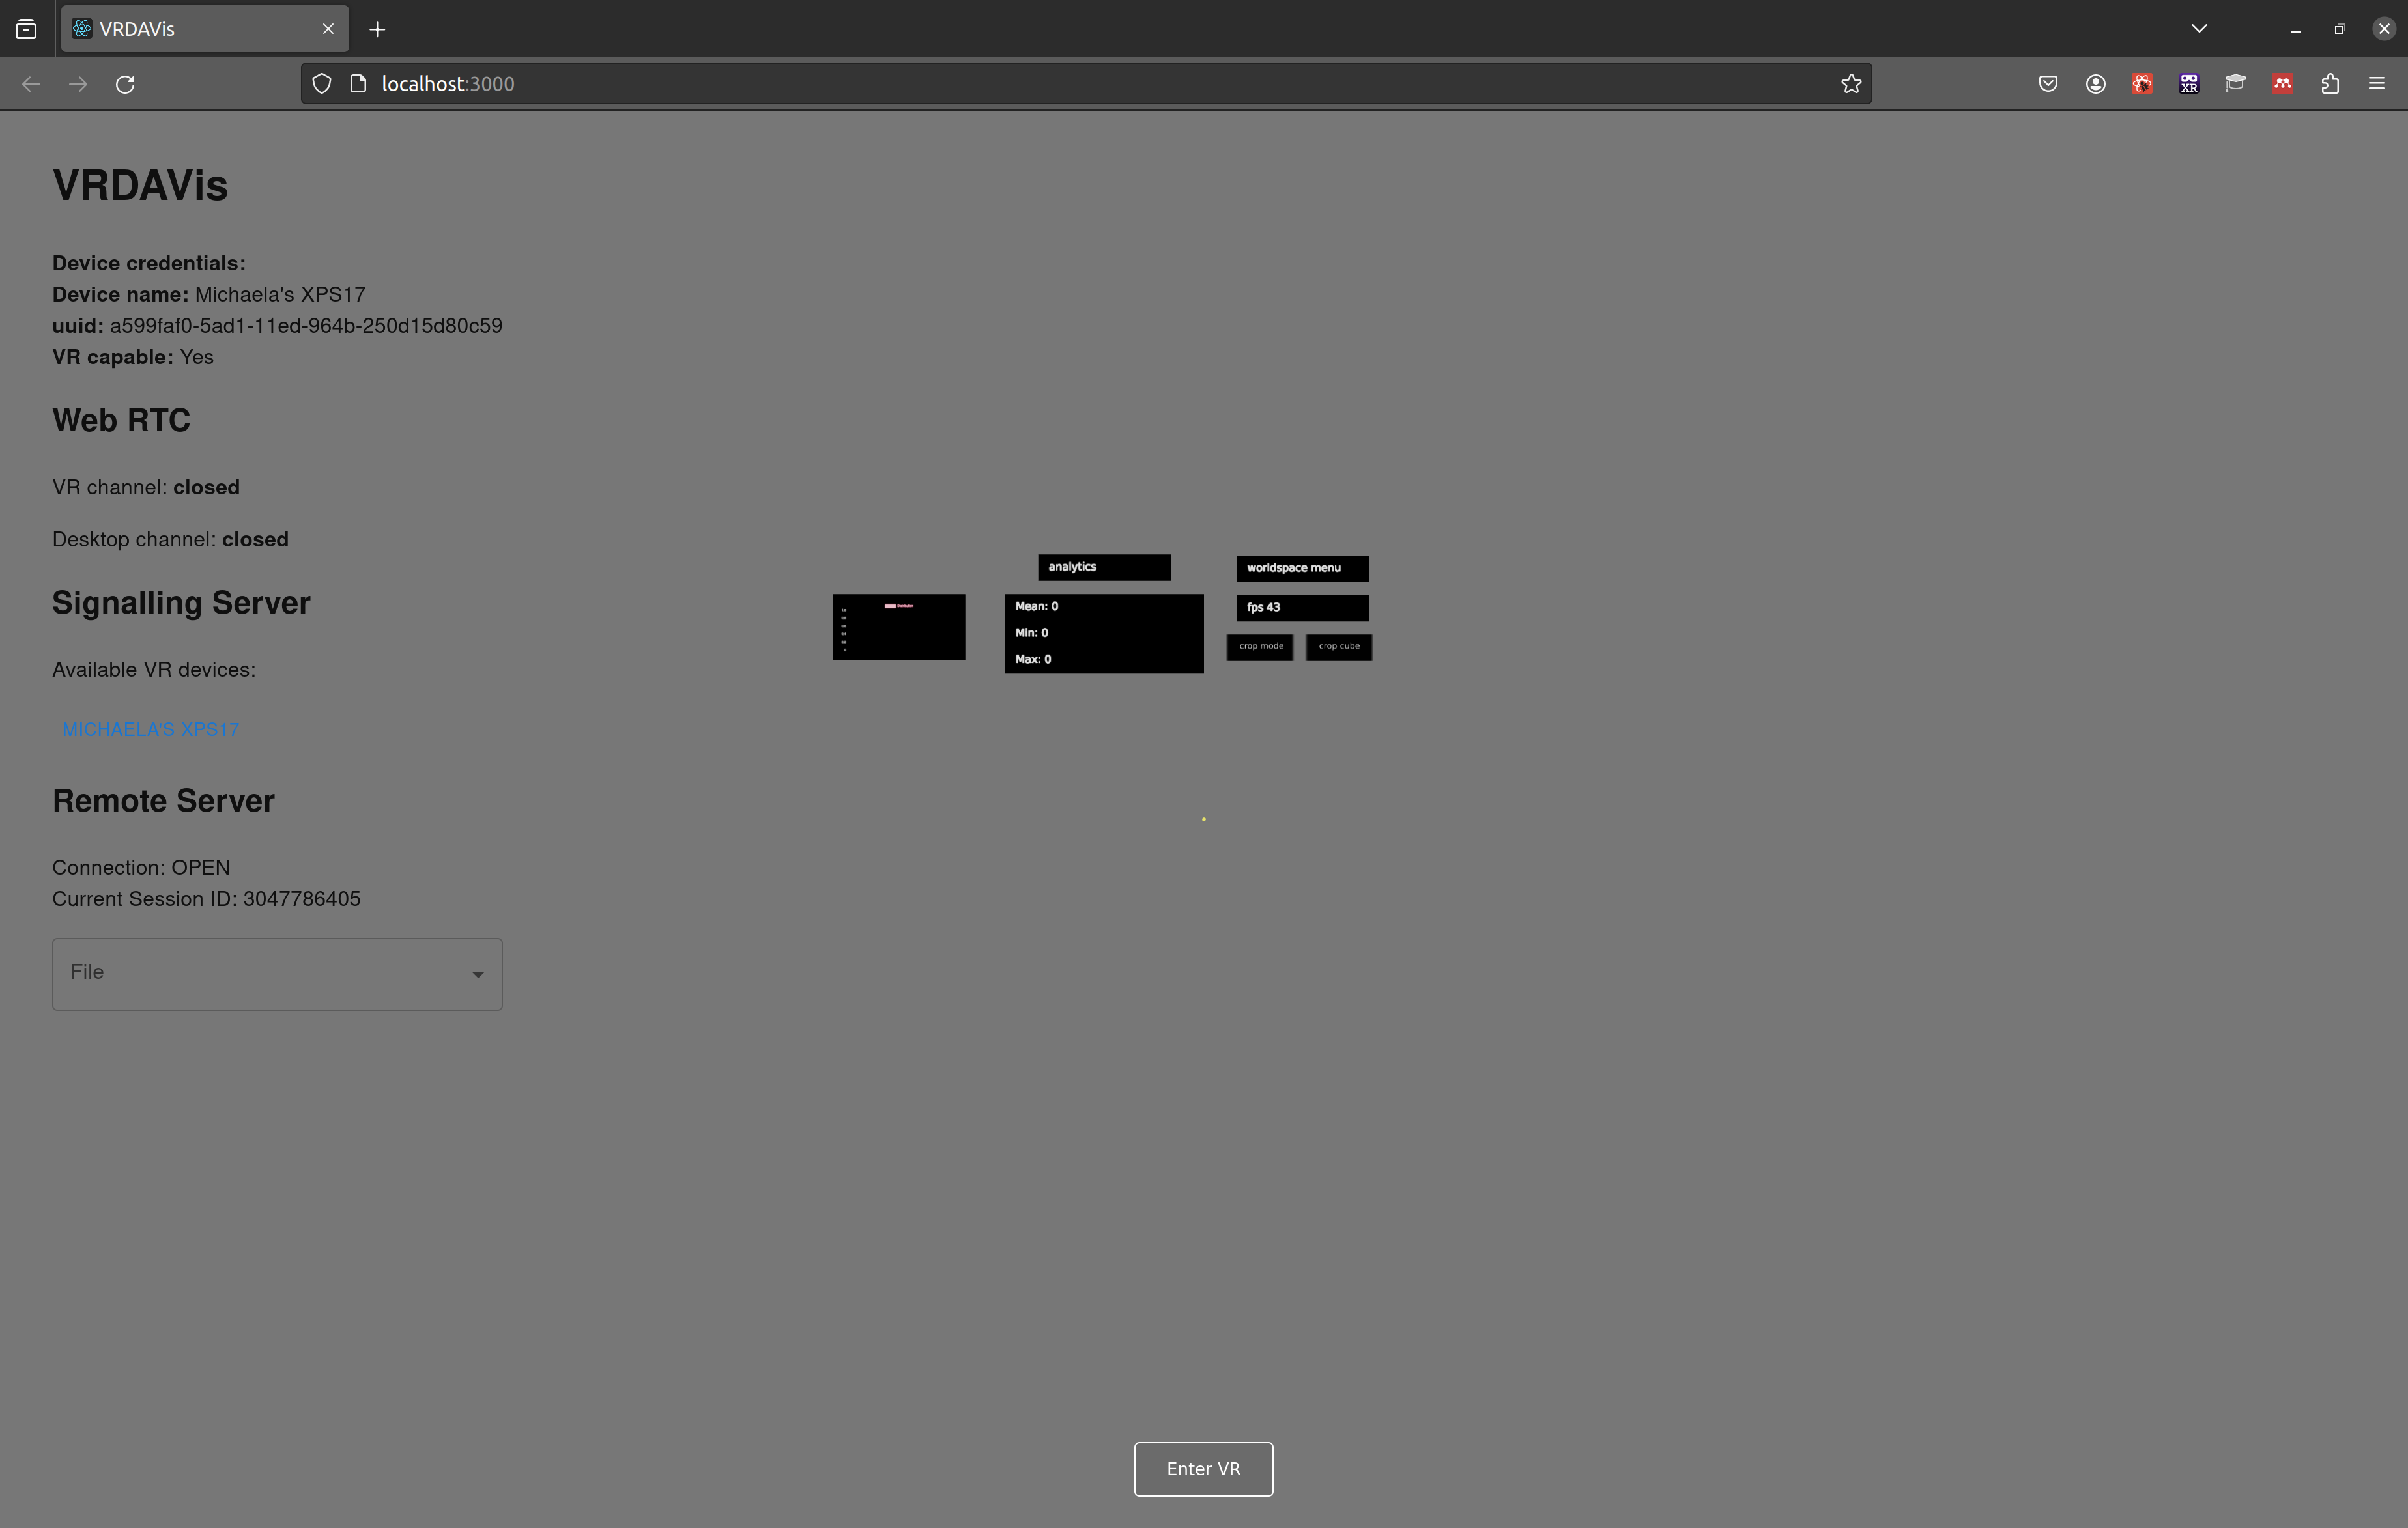
\includegraphics[width=\linewidth]{figures/screenshots/1.png}
    \caption{The appearance of the VRDAVis application when it is fist opened in the browser. In this instance the browser is Firefox. Some information about the current session can be seen on the left side of the screen, as well as the status of the peer-to-peer connection under the Web RTC heading, the available VR devices which can be paired with under the Signalling Server heading, and a drop down menu for selecting a data cubes under the Remote Server heading. Some VR environment assets can be seen in the centre of the screen.}
    \label{fig:screenshot-1}
\end{figure}

\begin{figure}
    \centering
    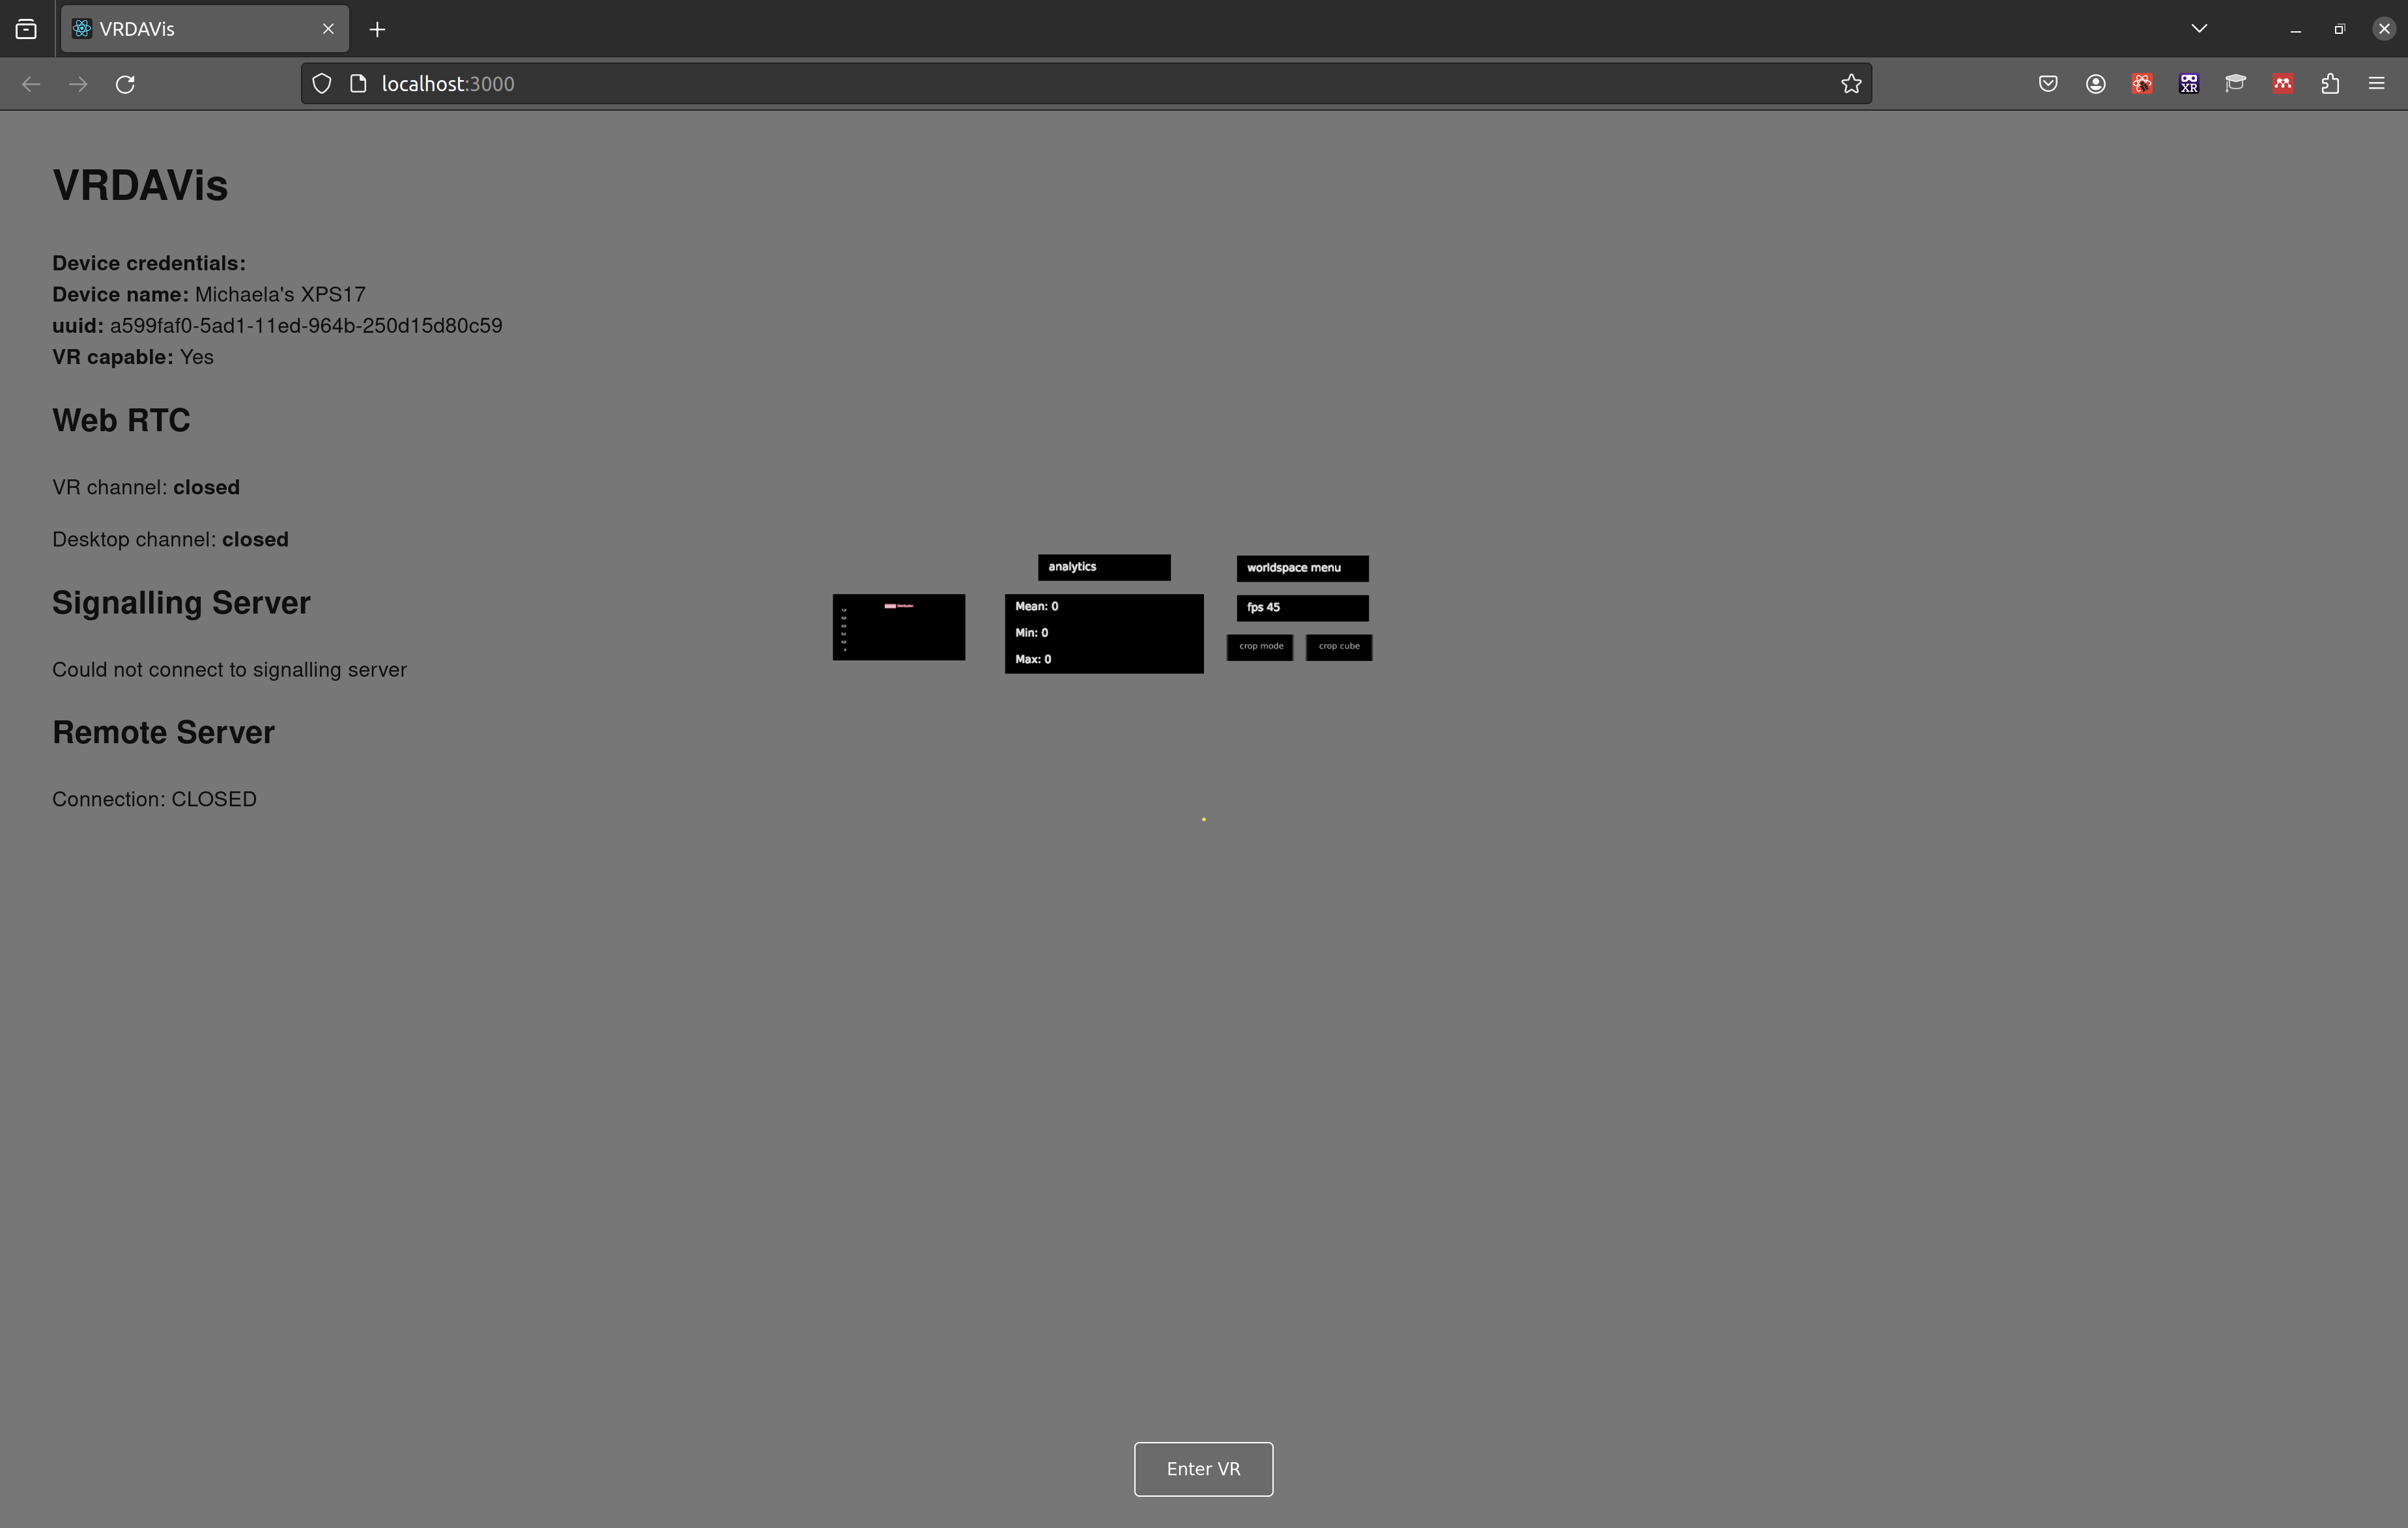
\includegraphics[width=\linewidth]{figures/screenshots/4.png}
    \caption{The appearance of the browser application when none of the remote services are available; there is no peer-to-peer connection, no connection to the signalling server, and no connection to the remote server.}
    \label{fig:screenshot-4}
\end{figure}

The data server sends the file list, and the user can choose which file they would like to explore. 
The user's file choice is sent to the data server, and the data server sends back some information pertaining to the selected file, such as dimensions and the size of the file. 
The client determines which cubelets it requires to generate the initial visualisation and requests them from the data server, while also specifying which analytics the data server needs to compute using the full-resolution data. 
The data server opens the file, reads the cubelets the client requested, compresses these cubelets into individual messages, and sends them to the client. 
Once the analytics are computed, they are also sent to the client.

When a cubelet reaches the client, it is decompressed and loaded into the GPU cache. 
The cubelet is then added to the three-dimensional, one at a time, until all the cubelets have been received and added. 
This three-dimensional texture is then rendered by the ray-casting shader.

\begin{figure}
    \centering
    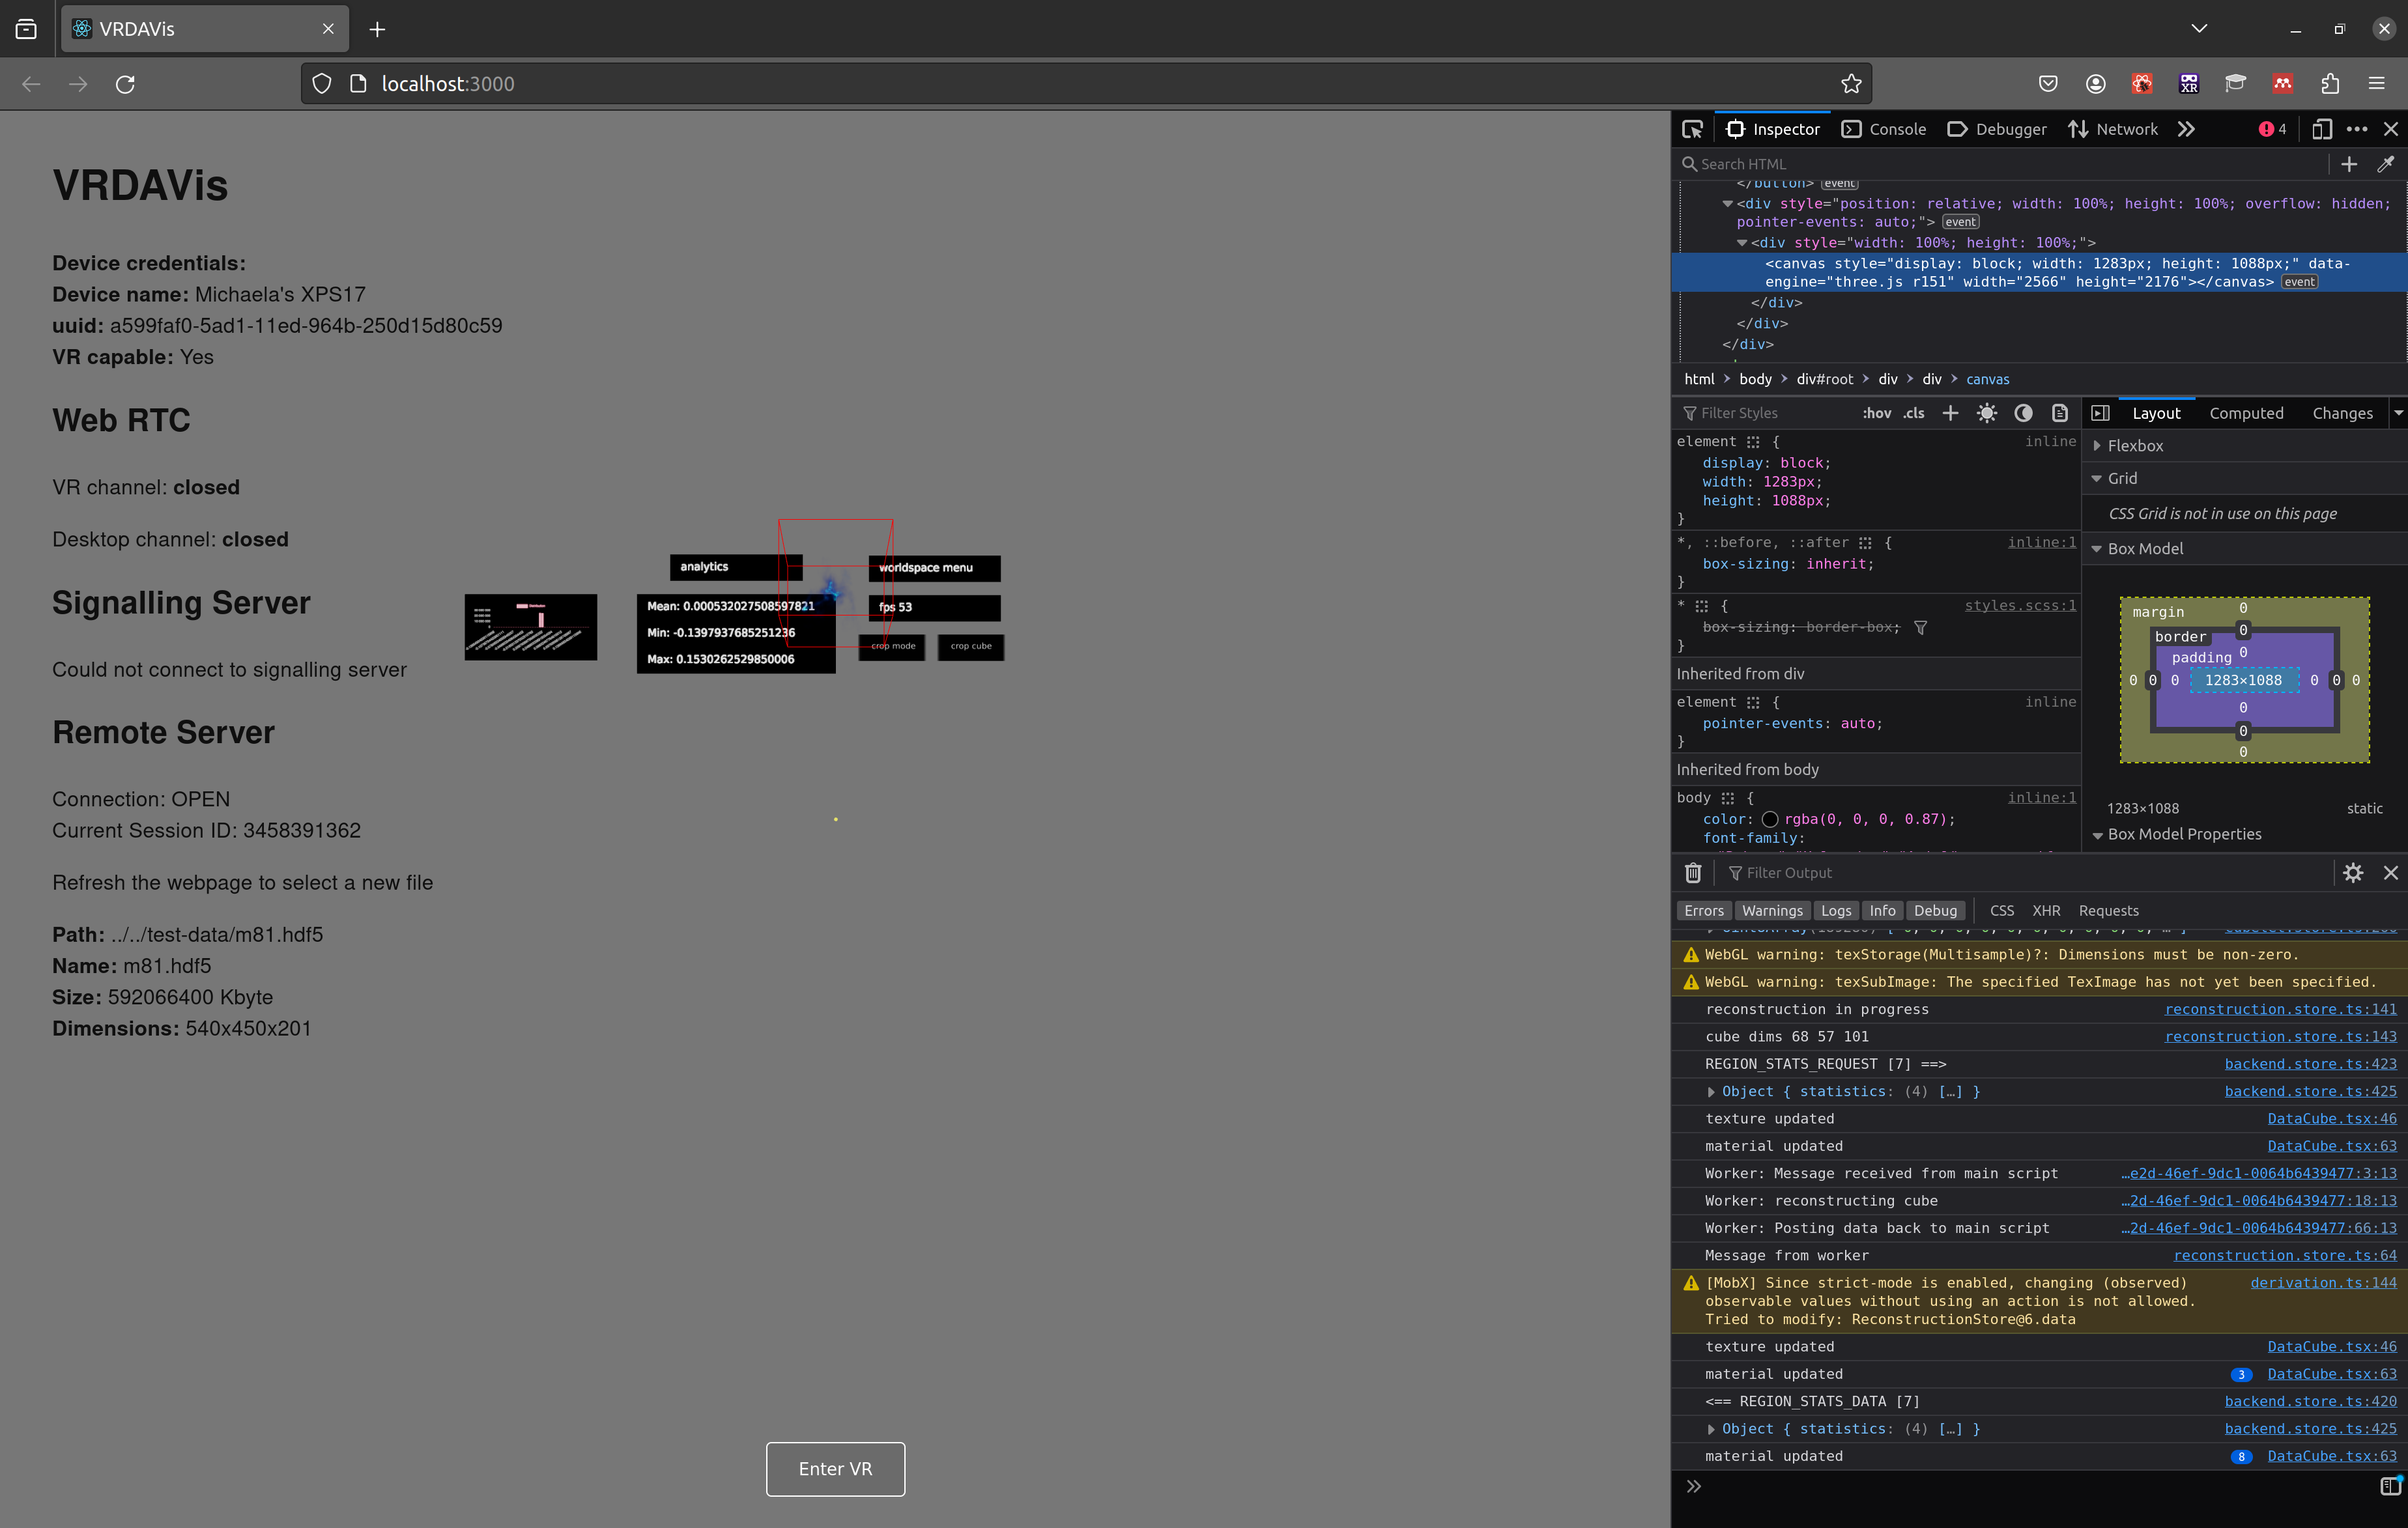
\includegraphics[width=\linewidth]{figures/screenshots/5.png}
    \caption{The view of the web browser application when a file has been selected and an initial visualisation of the data cube is within the VR environment. Some additional information about the data cube is displayed under the Remote Server heading; the path of the file on the remote server, the name of the file, the size in kilobytes, and the dimensions of the data cube.}
    \label{fig:screenshot-5}
\end{figure}

The user can then choose to switch to viewing the visualisation on the standalone VR headset. 
If the user switches to the headset, all the state information is sent over the peer-to-peer connection. 

The headset client uses the state information to start its own session on the data server and request the same cubelets as on the desktop client instance. 
The VR instance does not need the desktop instance to function; the user can choose to start the entire visualisation process on the VR headset by starting the client browser application on the browser. 
The main difference between the instance of the application on the desktop and the VR headset is that the VR headset client instance has the entry point to the VR environment, whereas the desktop does not have the capabilities to view a VR environment.

When the user enters the VR environment, they can interact with the visualisation in a three-dimensional space and view the analytics of the data. 
\begin{figure}
    \centering
    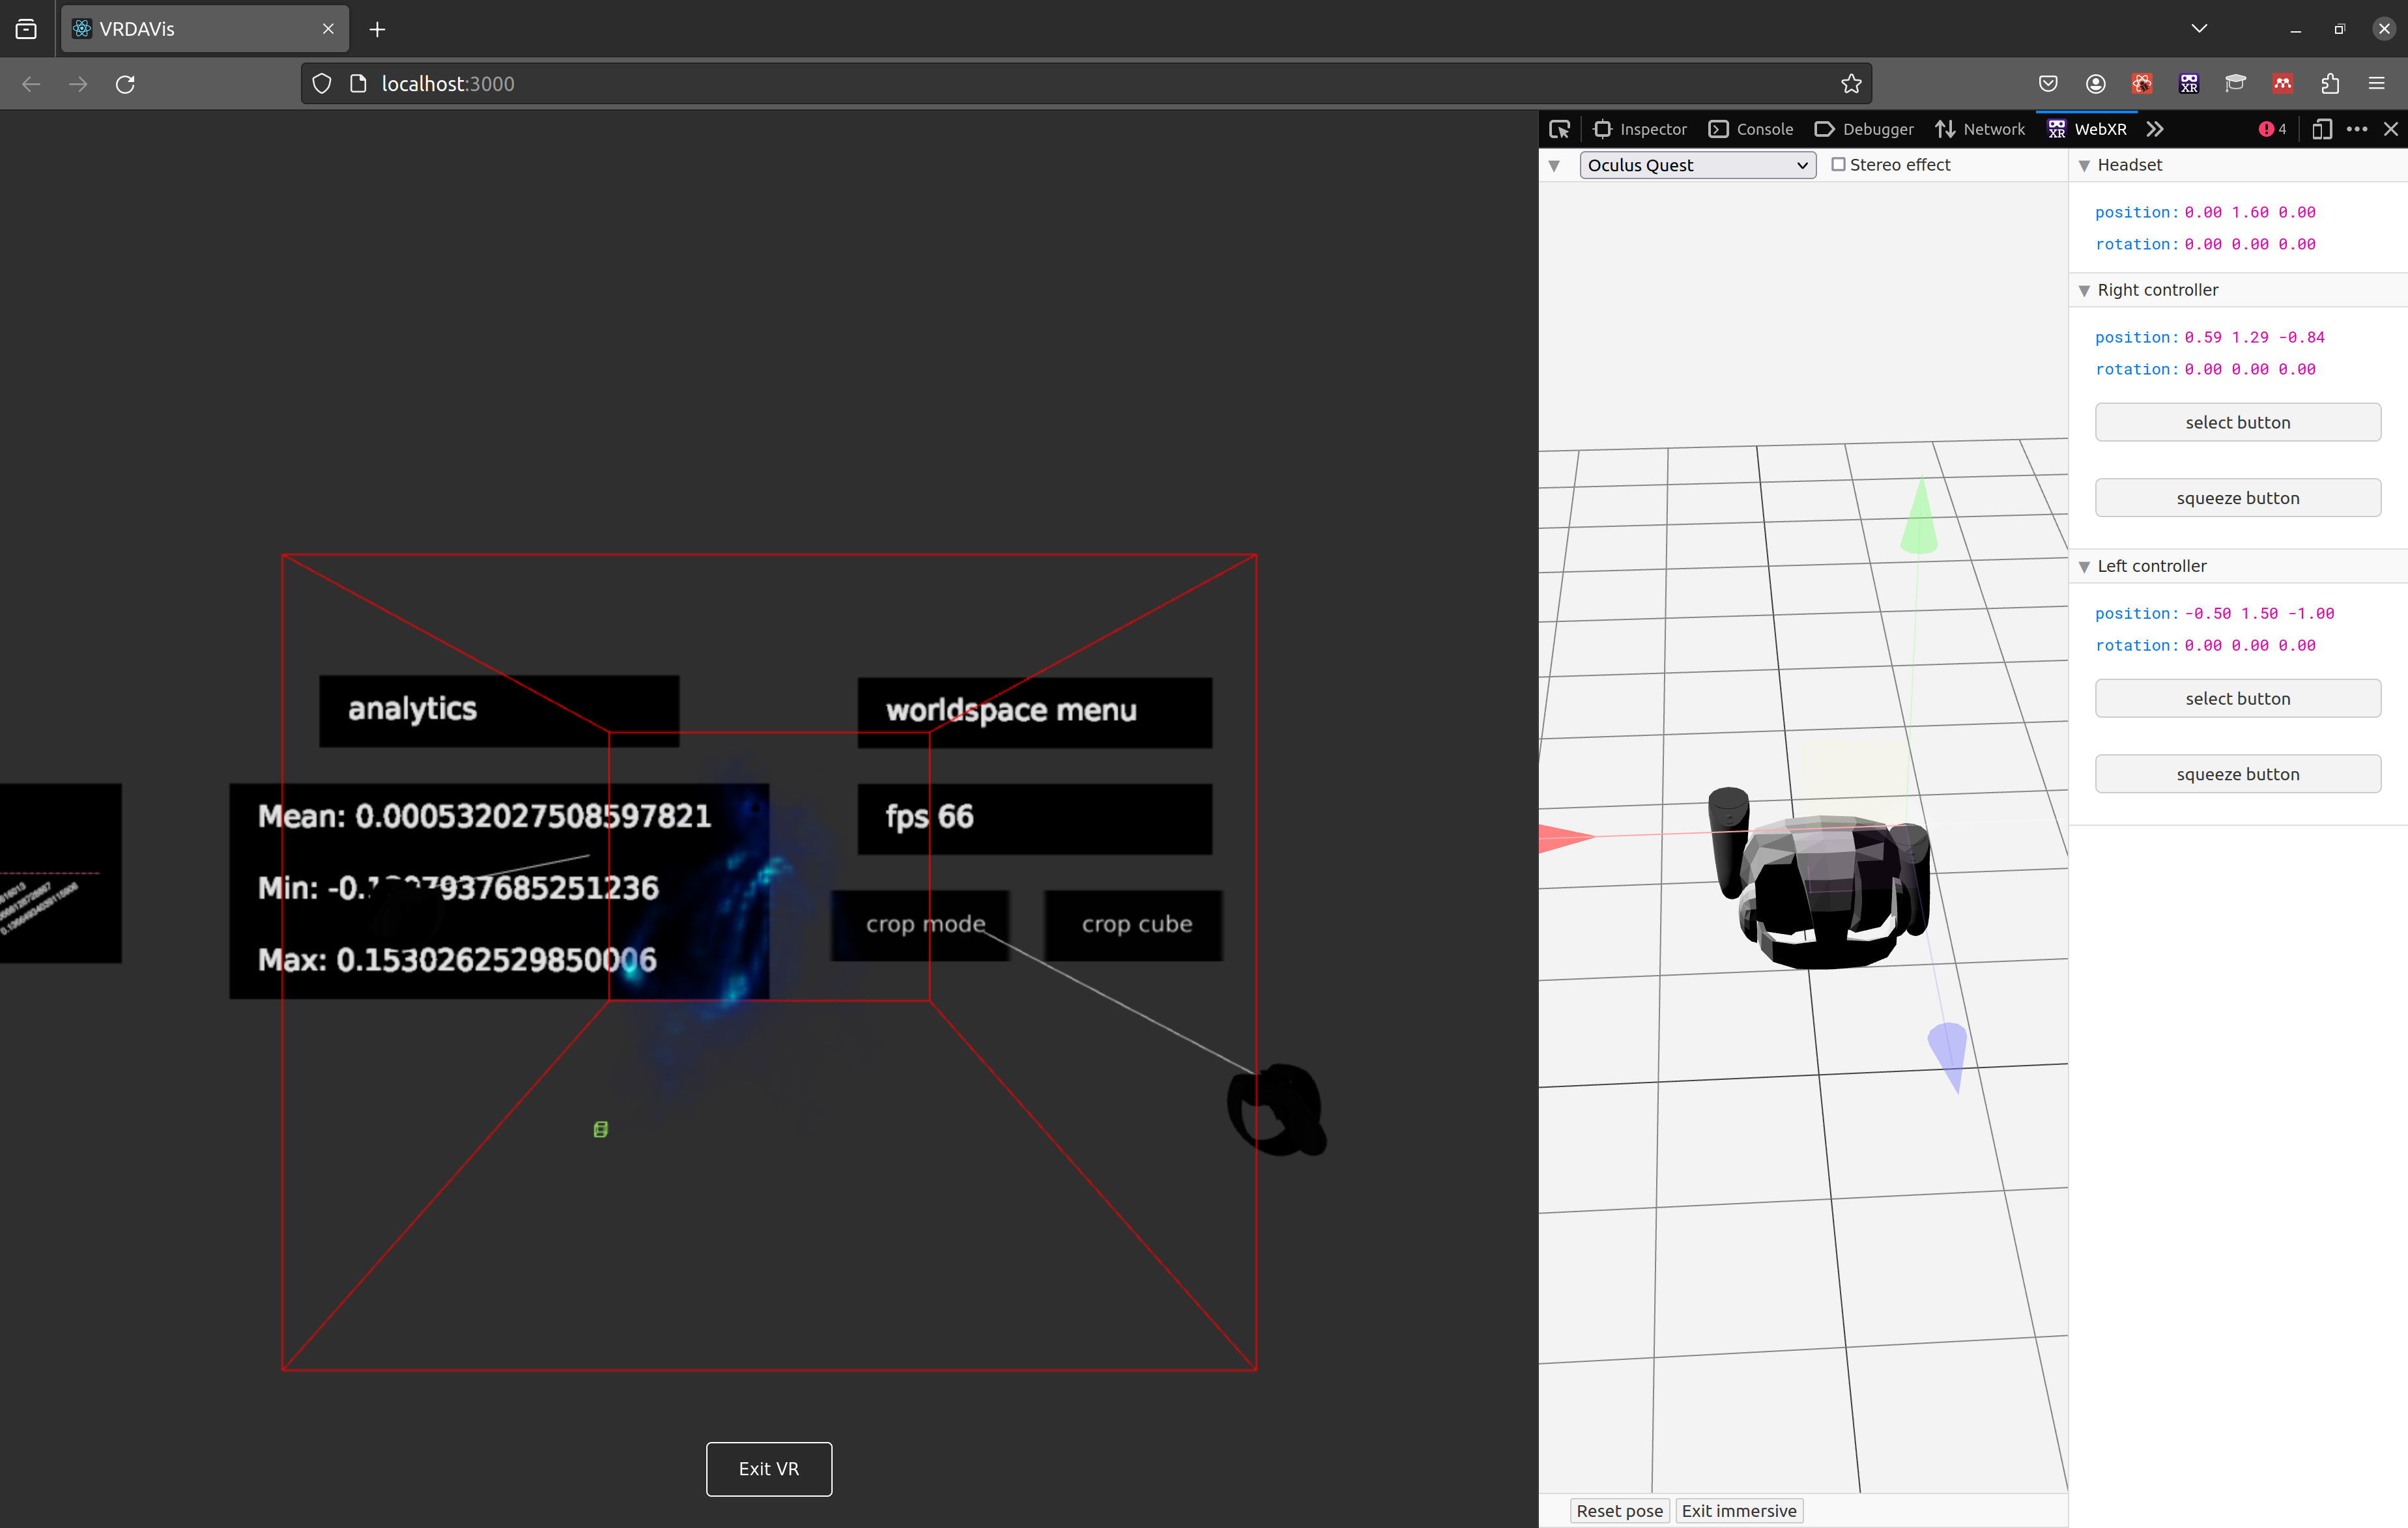
\includegraphics[width=\linewidth]{figures/screenshots/9.png}
    \caption{The view from inside the VR environment. The assets which could be seen on the centre of the view are now tangible within the VR environment. The data-cube is now a three-dimensional object and the analytics menu can be seen behind it. The WebXR browser plugin is used to view the VR environment from the browser window on a conventional screen. The plugin interface is displayed on the right side of the browser window.}
    \label{fig:screenshot-9}
\end{figure}
The user can crop the visualisation to get a higher-resolution version of the data by using the crop function; the user drags a box over the section they would like to take a closer look at and then selects the crop button. 
The client application determines which resolution level is appropriate for cubelet selection and sends a list of cubelets to the data server. 
The server fetches the cubelets and computes the analytics in the same way as it did for the initial visualisation. 
This process happens every time the cube is cropped until it reaches the highest resolution level, which is the full-resolution data. 
The size of the cubelets is determined by predetermined, internal values in the remote and front-end services.

\begin{figure}
    \centering
    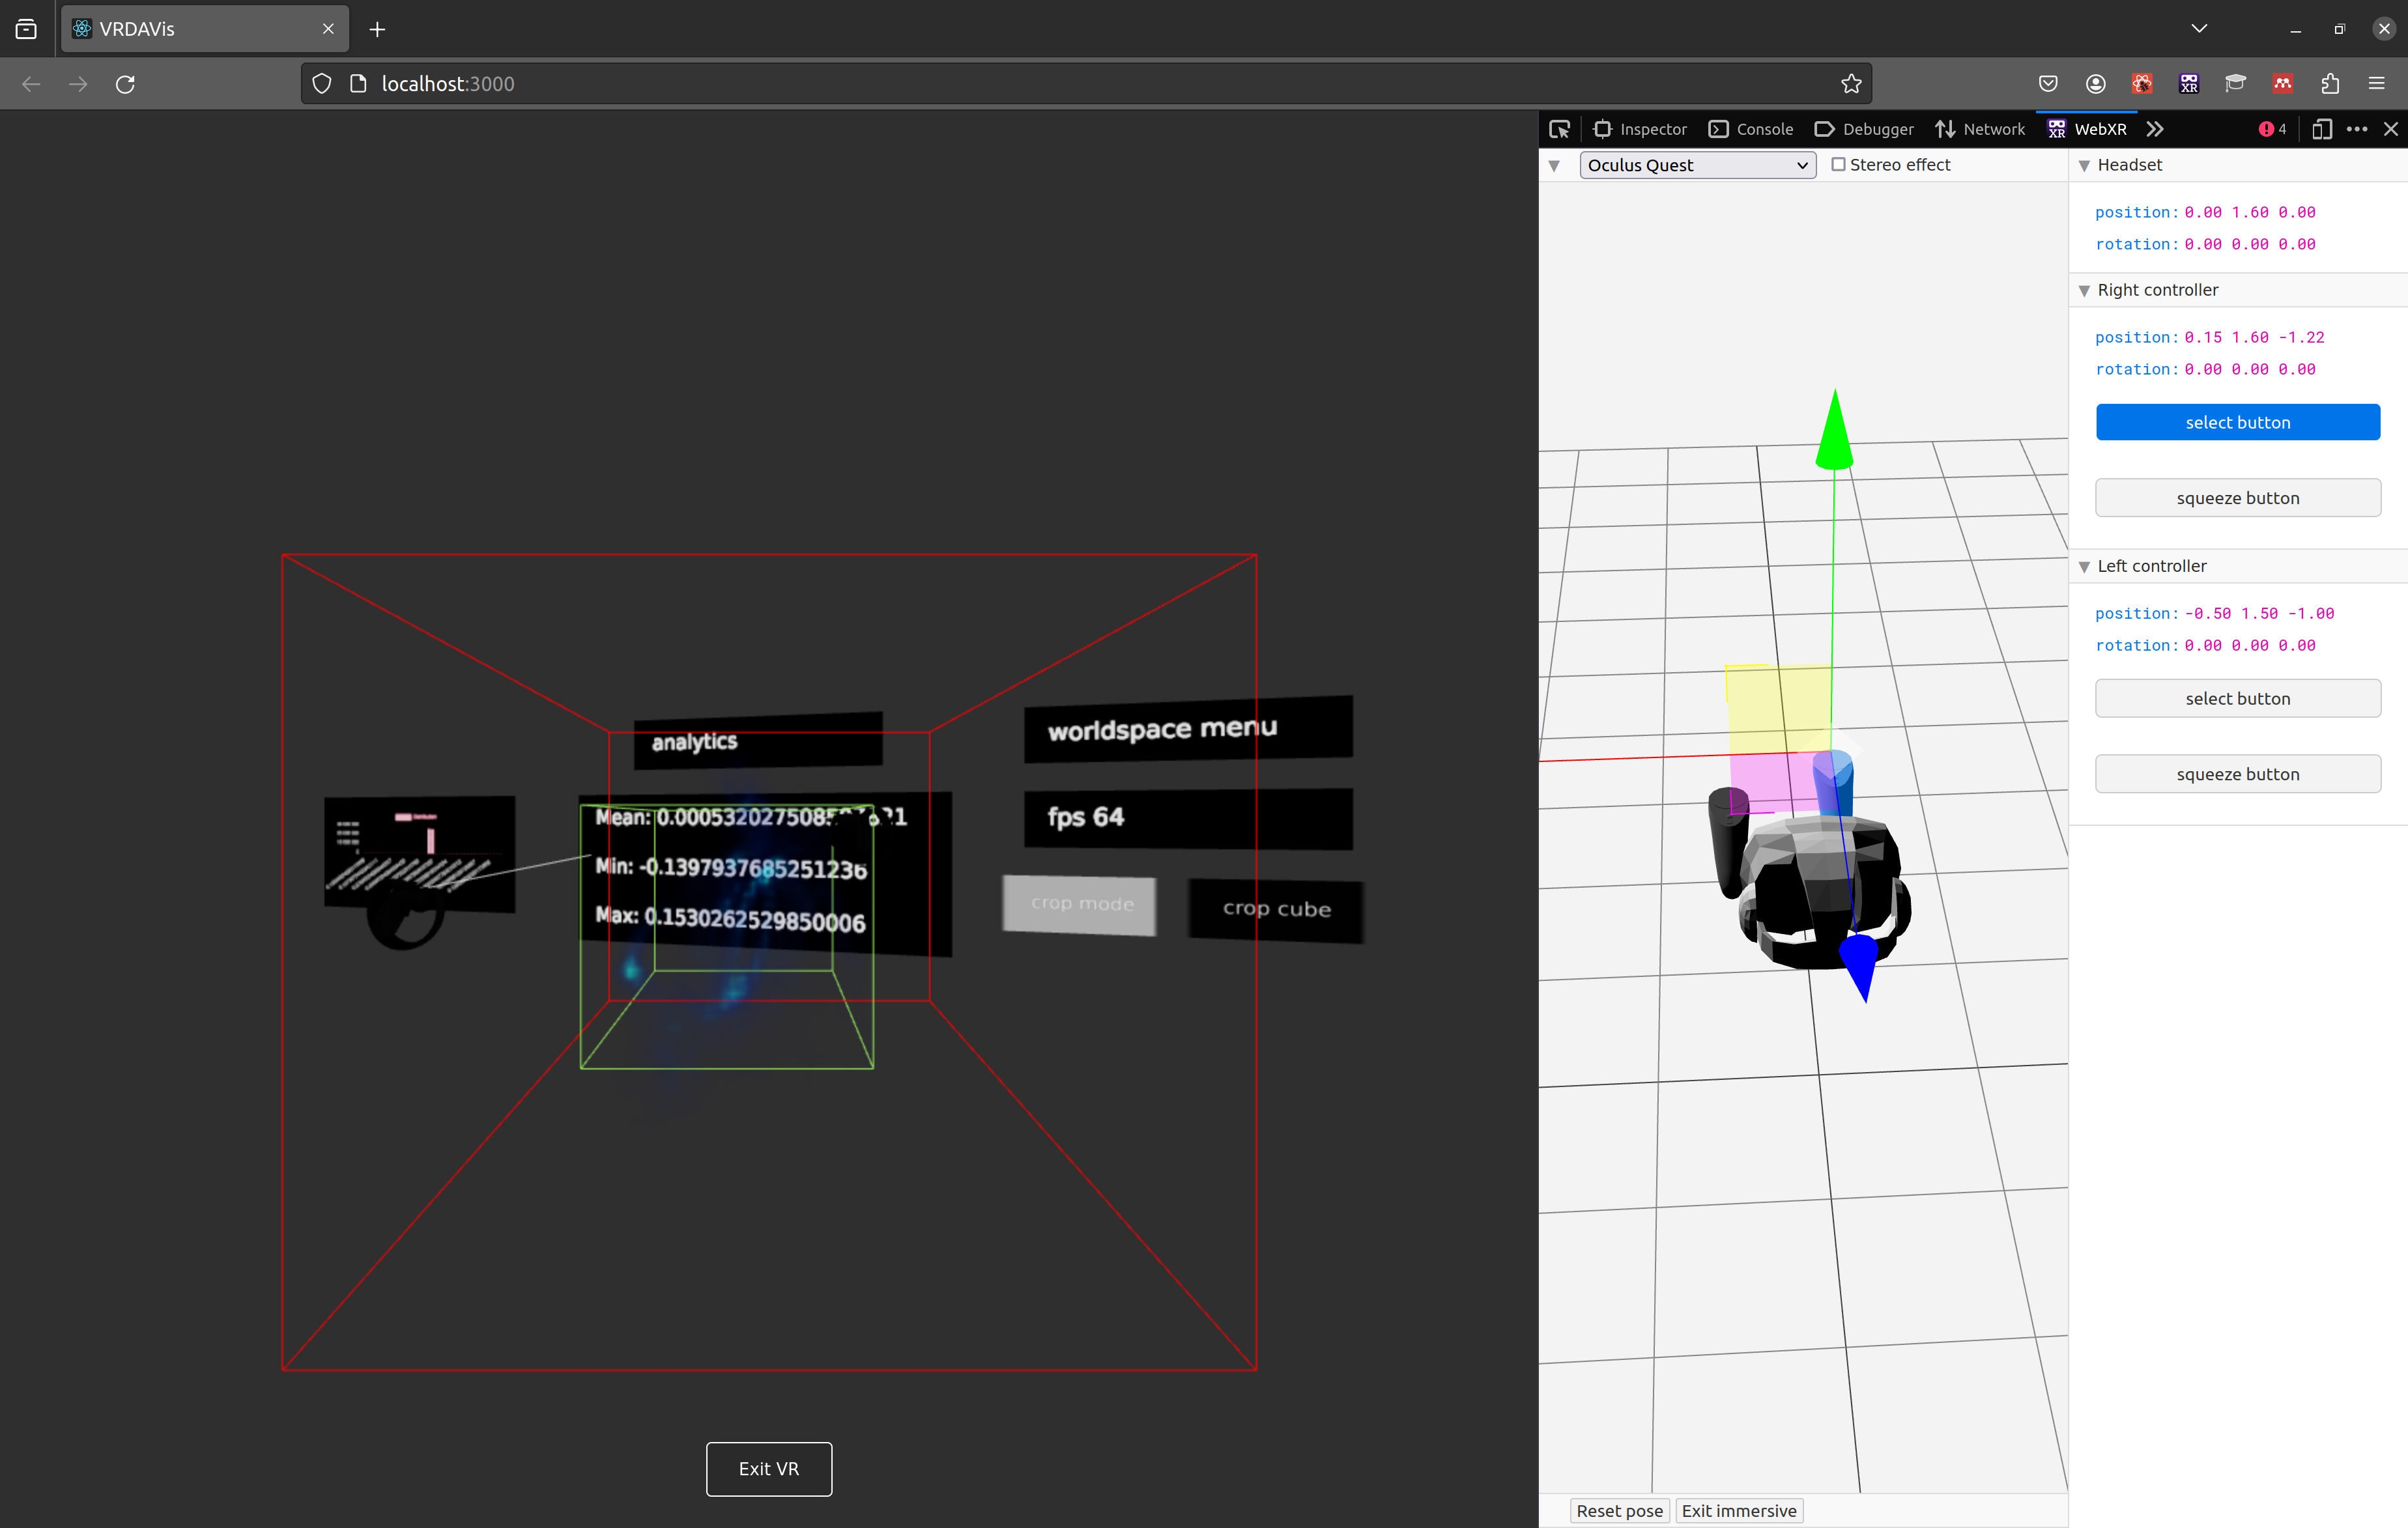
\includegraphics[width=\linewidth]{figures/screenshots/10.png}
    \caption{An example of a data cube displayed in the VR environment. The red cube represents an area within full dimensions of the data cube, and the green cube shows the selected crop area.}
    \label{fig:screenshot-10}
\end{figure}
